\chapter{Evaluation}\label{ch:evaluation}
% take a step back and put your results from 4 into context. 
This chapter conducts a comprehensive analysis of the \ac{ML} models implemented in
the preceding chapter.
An overview of the quality metrics used for the evaluation is presented in
Table~\ref{tab:evaluation_criteria}.
The quality metrics have been structures based on
the \ac{GQM}approach mentioned in subsection~\ref{subsec:goal-question-metric-approach}.

The quality metrics are aligned with the quality model
from~\cite{siebert2022construction}, which in turn is based on the ISO/IEC 9126 standard for
software quality evaluation.
The standard has been adapted by \cite{siebert2022construction} to meet the specific
requirements of machine learning models, as described in section~\ref{sec:evaluation-of-machine-
learning-models}.

As~\cite{siebert2022construction} mostly focuses on the evaluation of classification
models, the quality metrics have been adapted to fit the requirements of the regression
models implemented in this thesis.
This is elaborated in each individual quality metric section.

Table~\ref{tab:evaluation_criteria} shows the quality metrics used for the evaluation
of the \ac{ML} models.
The \ac{GQM} approach is used to structure the evaluation of the \ac{ML} models.
To each goal a question or one or more metrics where assigned.
The following subsections follow this structure and describe the quality metrics in more
detail.

\captionsetup{margin={5pt,5pt}}
\begin{table}[{}]
    \begin{tcolorbox}[arc=0pt,boxrule=0.5pt]
        \centering
        {\renewcommand{\arraystretch}{1}
            \begin{tabular}{p{2cm}p{8cm}p{3cm}}
                \toprule
                \thead{\textbf{Goal}} & \thead{\textbf{Question}}
                & \thead{\textbf{Metric}} \\
                \toprule
                \textbf{Correctness} & Ability of the model to perform the
                current task measured on the development dataset and the runtime dataset~\cite[p
                . 16]{siebert2022construction}
                &
                MAE, \newline MSE, \newline RMSE
                \\
                \hdashline
                \textbf{Relevance} & Does the model achieve a good bias-variance
                tradeoff? Which means neither overfitting or unterfitting the
                data.~\cite[p. 16]{siebert2022construction}
                & Variance of CV, \newline $R^2$
                \\
                \hdashline
                \textbf{Robustness} & Ability of the model to outliers, noise
                and other data quality issues~\cite[p. 16]{siebert2022construction}
                & Loss of Accuracy, \newline Average Loss
                \\
                \hdashline
                \textbf{Stability} & Does the artifact generate repeatable
                results when trained on different data?~\cite[p. 16]{siebert2022construction}
                & LOOCV stability
                \\
                \hdashline
                \textbf{Interpret- ability} & How well can the model be
                explained?~\cite[p. 16]{siebert2022construction}
                & Linearity, \newline monotonicity, \newline  interaction
                \\
                \hdashline
                \textbf{Resource utilization} & How much resources are
                required to train and run
                the model?~\cite[p. 16]{siebert2022construction}
                & Training time, \newline runtime, \newline storage space
                \\
                \bottomrule
            \end{tabular}
        } % renew command
    \end{tcolorbox}
    \caption{Overview of the goals, questions and metrics for the
    evaluation of artifacts
    following the \ac{GQM} approach.}
    \label{tab:evaluation_criteria}
\end{table}


\section{DP1: Correctness}\label{sec:dp1:-correctness}
% Ability of the model to perform the current task measured on the
% development dataset and the
% runtime dataset

The model must be able to perform well on the selected task.
\cite{siebert2022construction} used the classification metrics precision, recall and F-
score to evaluate the correctness models.
As the regression models implemented in this thesis are not able to predict
the class of a sample, these metrics are not applicable.

Commonly used metrics for regression models are the mean absolute error \ac{MAE},
\ac{MSE} and \ac{RMSE}.
Their formal description is given in~\ref{eq:mae},~\ref{eq:mse} and~\ref{eq:rmse} where
\(e_i\) being the prediction error which is the difference between the predicted value
by the model and the acutal value.
\(y_i\) is the actual value and \(n\) is the number of samples in the testing data set.

For the evaluatoins the \texttt{sci-kit learn}~(\cite{scikit-learn}) implementation of
these metric was
used.

\textbf{Mean Absolute Error (MAE)}

\begin{tcolorbox}[arc=0pt,boxrule=0.5pt]
    \begin{equation}
        MAE = \frac{1}{n} \sum_{i=1}^{n} |e_i|
        \label{eq:mae}
    \end{equation}
\end{tcolorbox}

The MSE is the average of the squared differences between the predicted and
the actual values.
The MSE is more sensitive to outliers than the MAE.

\textbf{Mean Squared Error (MSE)}

\begin{tcolorbox}[arc=0pt,boxrule=0.5pt]
    \begin{equation}
        \label{eq:mse}
        MSE = \frac{1}{n} \sum_{i=1}^{n} e^2
    \end{equation}
\end{tcolorbox}

The RMSE is the square root of the MSE. The RMSE is the most popular metric
for evaluating the
performance of regression models. The RMSE is interpretable in the same units
as the response
variable. The RMSE is more sensitive to outliers than the MAE.
The MAE is the average of the absolute difference between the predicted and
actual values.

\textbf{Root Mean Squared Error (RMSE)}

\begin{tcolorbox}[arc=0pt,boxrule=0.5pt]
    \begin{equation}
        \label{eq:rmse}
        RMSE = \sqrt{MSE}
    \end{equation}
\end{tcolorbox}

For a full overview about the performance all three metrics are sued for the
evaluation.

% \subsection{Goal Hierarchy}

% The correctness describes the ability of the model to perform on the
% selected task. Concrete,
% the model has to predict the spring back as correct as possible. The goal
% hierarchy for the
% correctness is shown in Figure~\ref{fig:goal_hierarchie_correctness}.

% \begin{figure}[H]
%     \centering
%     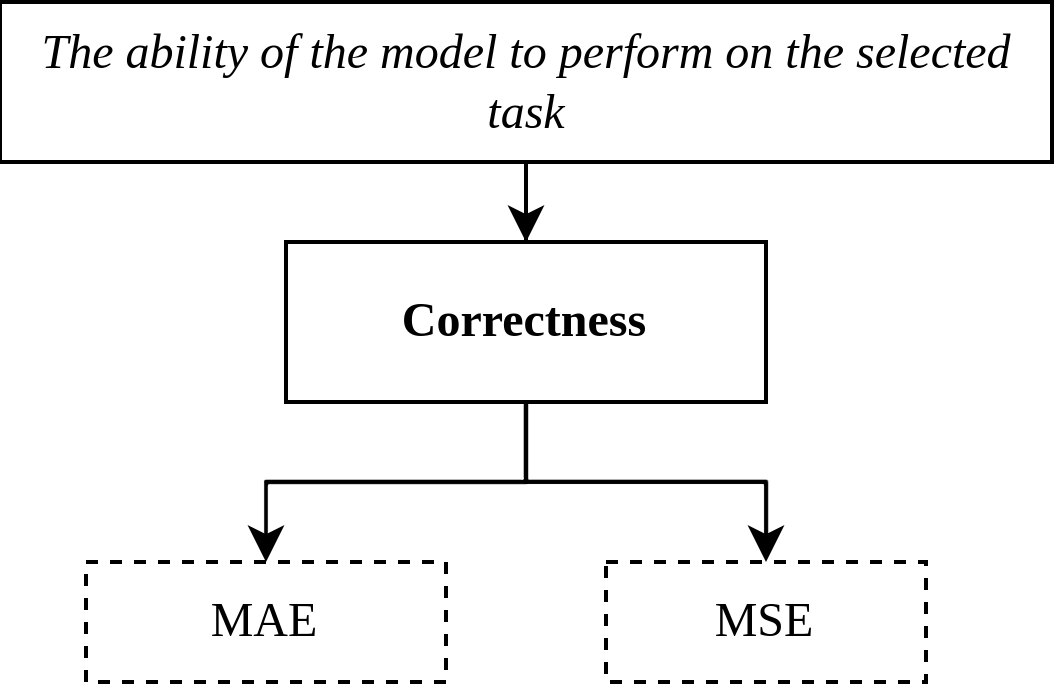
\includegraphics[width=0.6\textwidth]{goal_hierarchie_correctness}
%     \caption{Goal hierarchy: Correctness}
%     \label{fig:goal_hierarchie_correctness}
% \end{figure}

\subsection{Results}\label{subsec:results}
The Table~\ref{tab:results-correctness} shows the results of the
evaluation of the models for the correctness.

Looking at the \ac{RMSE} all models except the \ac{LR} and \ac{DC} models show a
relatively equal performance.
The \ac{MLP} has a slight advantage over the other models, with an \ac{RMSE} of 0.201.
Therefore it could be interesting to investigate the performance of neural networks /
deep learning in the future.

It's worth mentioning that the \ac{SVM} model has a slightly better \ac{MAE}, while
still maintaining a comparable \ac{MSE} compared to the other models.
This could be due to the fact that the errors made by the \ac{SVM} are evenly
distributed across instances, or that the errors made by the other models are large for
a few instances but smaller for the rest.

The algorithms \ac{LR} does perform worse than the other models.
A likely reason is, that the relationship between the independent and dependent
variables is not linear.
This can result in an inadequate fit and reduced predictive power (Source).

\ac{DT} on the other hand, can perform poorely when they overfit the training data.
Also, they are pron to instability, both problems are mitigates by using ensemble methods
like \ac{RF} and \ac{GBT} which can overcome the limitations of individual
decision trees.

Because the simple \ac{DT} as well as the \ac{LR} are not able to predict the
spring back correctly, they are not considered for the next steps of the evaluation.

% Table wit hall used machine learning models and their metrics
\begin{table}[H]
    \begin{tcolorbox}[arc=0pt,boxrule=0.5pt]
% \sisetup{group-minimum-digits = 4}
        \centering
        \begin{tabular}{llll}
            \toprule
            \thead{\textbf{Model Name}} & \thead{\textbf{MAE}}
            & \thead{\textbf{MSE}}
            & \thead{\textbf{RMSE}} \\
            \toprule
            \textbf{LR}  & 0.199 & 0.092 & 0.303 \\
            \hdashline
            \textbf{DT}  & 0.193 & 0.076 & 0.266 \\
            \hdashline
            \textbf{RF}  & 0.183 & 0.060 & 0.244 \\
            \hdashline
            \textbf{ET}  & 0.126 & 0.040 & 0.201 \\
            \hdashline
            \textbf{AB}  & 0.163 & 0.040 & 0.209 \\
            \hdashline
            \textbf{GBT} & 0.189 & 0.058 & 0.242 \\
            \hdashline
            \textbf{SVM} & 0.09  & 0.04  & 0.20  \\
            \hdashline
            \textbf{MLP} & 0.114 & 0.041 & 0.201 \\
            \bottomrule
        \end{tabular}
        \caption{Overview of the used machine learning models and their
        metrics.}
        \label{tab:results-correctness}
    \end{tcolorbox}
\end{table}


\section{DP2: Relevance}\label{sec:relevance}
% Does the model achieve a good bias-variance tradeoff? Which means neither
% overfitting or
% unterfitting the data.

% Bias variane trade-off
A model is considered relevant when it achieves a balance between bias and
variance, avoiding both overfitting and underfitting of the training data.
The relevance of the model can be quantified through the \textit{variance of
cross-validation}, which proves insight into how the model performs when trained and
evaluated on different subsets of data and how generalizes.

% Explanation interpretation of variance
A low variance indicates that the model's performance is consistent across
different folds,suggesting that the model is not overfitting the training data.
Conversely, a high variance implies that the performance can vary significantly
depending on the specific data points used the test set, indicating a potential
overfitting problem.

Cross validations was explained in Section~\ref{subsec:cross-validation}.
As estimator for the trained model $R^2$ was used which is a statistical measure of how close the
data is to the fitted regression line (this makes no sense).

Equation~\eqref{eq:r2} shows the formula for the $R^2$ score:

\begin{equation}
    \label{eq:r2}
    R^2 = \frac{Explained\_variance}{Total\_variance\_targert\_variable}
\end{equation}

The value of the \(R^2\) is the percentage of the response variable variation that is
explained by a linear model.
It returns a score between 0 and 1, where 0 means that the model does not
explain any of the variance in the response variable around its mean, and 1 means that
the model explains all the variance in the response variable around its mean~\cite[p.
43]{muller_introductionmachinelearning_2016}.
Special in sci-kit learns implementations is that the score can be negative if the model
performs poorly.
If a model always predicts the expected value of y, regardless of the
input features, it would receive an R^2 score of 0.0~\cite{_sklearnmetricsr2_}.

Therefore, a high \(R^2\) indicated a good model fir and good bias-variance
tradeoff\cite[p. 43]{muller_introductionmachinelearning_2016}.

\subsection{Results}\label{subsec:results3}

Table~\ref*{tab:results_relevance} shows the variance of cross-validation
and the \(R^2\) for all used machine learning models.
To calculate the variance of cross-validation the variance of Scikit-Learn's
\texttt{cross\_val\_score} was calculated.
Five-fold cross-validation was used to calculate the variance of
cross-validation.
The \(R^2\) was calculated with the formula~\ref{eq:r2}.

It can be observed that most of the models have relatively low variance, indicating
consistent performance across different folds, however, two models stand out - \ac{GBT}
and ac{MLP}.

For the \ac{GBT} model, the variance is high, which implies that its performance
fluctuates significantly across different folds.
This inconsistency is a typical sign of overfitting, where the model is overly complex
and has learned the noise in the data rather than the underlying pattern.
The individual cross-validation scores for the GBT model also confirm this assumption,
with a negative score on the first fold and relatively high scores on the subsequent
folds.
Given this poor performance, the GBT model cannot be considered relevant for the given
task.

Similarly, the \ac{MLP} model has a relatively high variance score, which suggests that
its performance also fluctuates across different folds. The individual scores for the MLP
model show that it performs poorly on a few folds.

This performance inconsistency could be due to either overfitting or high variability
in the data.

Overall, it's important to consider the cross-validation scores in conjunction with
the other other metrics to get a more complete picture of how well your model is
performing.
This will be done in later sections.

\begin{table}[H]
    \begin{tcolorbox}[arc=0pt,boxrule=0.5pt]
% \sisetup{group-minimum-digits = 4}
        \centering
        \begin{tabular}{llll}
            \toprule
            \thead{\textbf{Model Name}} & rs & \thead{\textbf{Variance of CV}}
            & \thead{\textbf{\(R^2\)}} \\
            \toprule
            \textbf{RF}  & - & 0.068 & 0.8   \\
            \textbf{RF}  & x & 0.071 & 0.805 \\
            \hdashline
            \textbf{ET}  & - & 0.064 & 0.832 \\
            \textbf{ET}  & x & 0.352 & 0.82  \\
            \hdashline
            \textbf{GBT} & - & 0.425 & 0.775 \\
            \textbf{GBT} & x & 0.426 & 0.866 \\
            \hdashline
            \textbf{SVM} & - & 0.061 & 0.838 \\
            \textbf{SVM} & x & 0.061 & 0.798 \\
            \hdashline
            \textbf{MLP} & - & 0.146 & 0.839 \\
            \textbf{MLP} & x & 0.146 & 0.871 \\
            \bottomrule
        \end{tabular}
        \caption{Performance of the used machine learning models according
        relevance.}
        \label{tab:results_relevance}
    \end{tcolorbox}
\end{table}


\section{DP3: Robustness}\label{sec:robustness}
% Ability of the model to outliers, noise and other data quality issues
% Variance of cross-validation, fit

%It should be noted that the original definition of the ``Robustness`` metric was limited
%to classification models.
%To address this limitation, the definition of the metric has been altered to fit the
%requirements of the regression models implemented in this thesis. This is further
%described
%in the section ``Robustness``~\ref{sec:robustness}.

% Also sibert et all uses Equalized Loss of Accuracy (ELA) which was changed

% Definition of robustness
The IEEE standard glossary of software engineering terminology describe
robustness as ``The degree
to which a system or component can function correctly in the presence of
invalid inputs or
stressful environmental conditions''~\cite[p. 64]{terminology1990ieee}.
\cite{saez2016evaluating} extend this definition to fit machine learning
models and describe it
as the ``capability of an algorithm to build models that are insensitive to
data corruptions and
suffer less from the impact of noise''~\cite[p.
2]{saez_evaluatingclassifierbehavior_2016}.
\cite{siebert2022construction} specifically mention data quality issued like
outliers or noise~\cite[p. 16]{siebert2022construction}.

Unlike \ac{DP} Correctness(\ref{sec:dp1:-correctness}), robustness is a
non-functional characteristic of a \ac{ML} model.
A way to evaluate the robustness is to check the correctness of the model with
added noise to the data~\cite[p. 18]{zhou_machinelearning_2021}, if the model
is still able to predict the correct values, it is considered robust.

As mentioned in section~\ref{subsec:dataset-exploration} the data set
was generated in a controlled environment does not contain many data quality
issues and noise.
This offers the opportunity to test the robustness of the models by manipulating the
data set to introduce the data quality issues missing values and noise.

\subsection{Missing Data}\label{subsec:missing-data}
When applying the model to real-world data, it is possible that some values
are missing.
Looking at the available dataset two scenarios or missing data can occur:
Missing \(Vt\)-pairings and missing values.

In the first scenario, there may be no data available for a specific die
opening, which can be due to the die opening was never being used before or a
lack of recorded
information.
In the second scenario, while data may exist for the desired \(Vt\)
combination, certain values may
be missing or the dataset may not be complete.

To address these scenarios, the following tests were conducted:

\subsubsection{Missing values}
%To assess the ability of the model to handle missing data, three experiments were
%conducted.

Initially, the use of the \ac{LPOCV} method was considered.
However, this approach was omitted due to computational constraints, as it generates all possible
training and test sets by removing \(p\)samples from the complete dataset, resulting in a large
number of overlapping test sets and a high computational cost.

As an alternative, regular \ac{CV} was applied, with an increasing number of folds.
The minimum number of folds was 2 and the maximum was equal to the total number of samples in the
dataset.
However, this experiment did not provide distinguishable results and was therefore not
included in the results.

The third and final experiment utilized random sampling to create different train-
test data compositions, allowing for the evaluation of the model's handling of missing data.
Split rations from 90:10 to 10:90 were used, with a step size of 10. This approach was inspired by a
similar method used in a previous study~\cite[p. 570--574]{liu2021deep}  which used thee different
split ratios to evaluate the performance of a deep learning model.


The results of this experiment provided valuable insights into the model's performance under
different data compositions, particularly when dealing with missing
data, and were used in conjunction with other metrics to gain a comprehensive understanding of
the model's overall performance.

%\begin{table}[H]
%    \begin{tcolorbox}[arc=0pt,boxrule=0.5pt]
%% \sisetup{group-minimum-digits = 4}
%        \centering
%        \begin{tabular}{lllll}
%            \toprule
%            \thead{\textbf{Model }} & rp &
%                {\thead{\textbf{80\% train} \\ \unit{MSE}}} &
%                {\thead{\textbf{50\%train} \\ \unit{MSE}}} &
%                {\thead{\textbf{20\%train} \\ \unit{MSE}}}
%            \\
%            \toprule
%            \textbf{RF} & - & 0.106 & 0
%            .099 & 0.012 \\
%            \textbf{RF} & x & 0.064 & 0
%            .089 & 0.114 \\
%            \hdashline
%            \textbf{ET} & - & 0.75 & 0
%            .116 & 0.094 \\
%            \textbf{ET} & x & 0.059 & 0
%            .093 & 0.079 \\
%            \hdashline
%            \textbf{GBT} & - & 0.045 & 0
%            .055 & 0.069 \\
%            \textbf{GBT} & x & 0.045 & 0
%            .055 & 0.069 \\
%            \hdashline
%            \textbf{SVM} & - & 0.071 & 0
%            .086 & 0.074 \\
%            \textbf{SVM} & x & 0.071 & 0
%            .086 & 0.074 \\
%            \hdashline
%            \textbf{MLP} & - & 0.053 & 0.057 & 0.45 \\
%            \textbf{MLP} & x & 0.053 & 0.057 & 0.54 \\
%            \bottomrule
%        \end{tabular}
%        \label{tab:ml_models_relevance}
%    \end{tcolorbox}
%    \caption{Performance of the used machine learning models according
%    relevance.}
%\end{table}

Figure~\ref{fig:results-missing-values} shows how the models performed when trained on
continuously less data.

It can be seen that all models perform well when trained with on 90\% of the data.
However, when trained on 50\% of the data, the \ac{MLP}  and \ac{GBT} models start to perform
better than the
other models.
When trained on 20\% of the data and less all models significantly underperform.
Also the \ac{ET} model stays relatively stable when trained on less data.

Looking at the variances the the \ac{SVM} and \ac{MLP} models perform the and seem to be the most
robust models when trained on less data.
It has to be noted, that as seen in sub-figure (a) the most variances comes from training on
below 20\% of the data.

Overall the \ac{MLP} model seems to be the most robust model, as it performs well on all data
compositions and has the lowest variance.

\begin{figure}[H]
    \begin{tcolorbox}[arc=0pt,boxrule=0.5pt]
        \centering
        \begin{subfigure}{0.4\textwidth}
            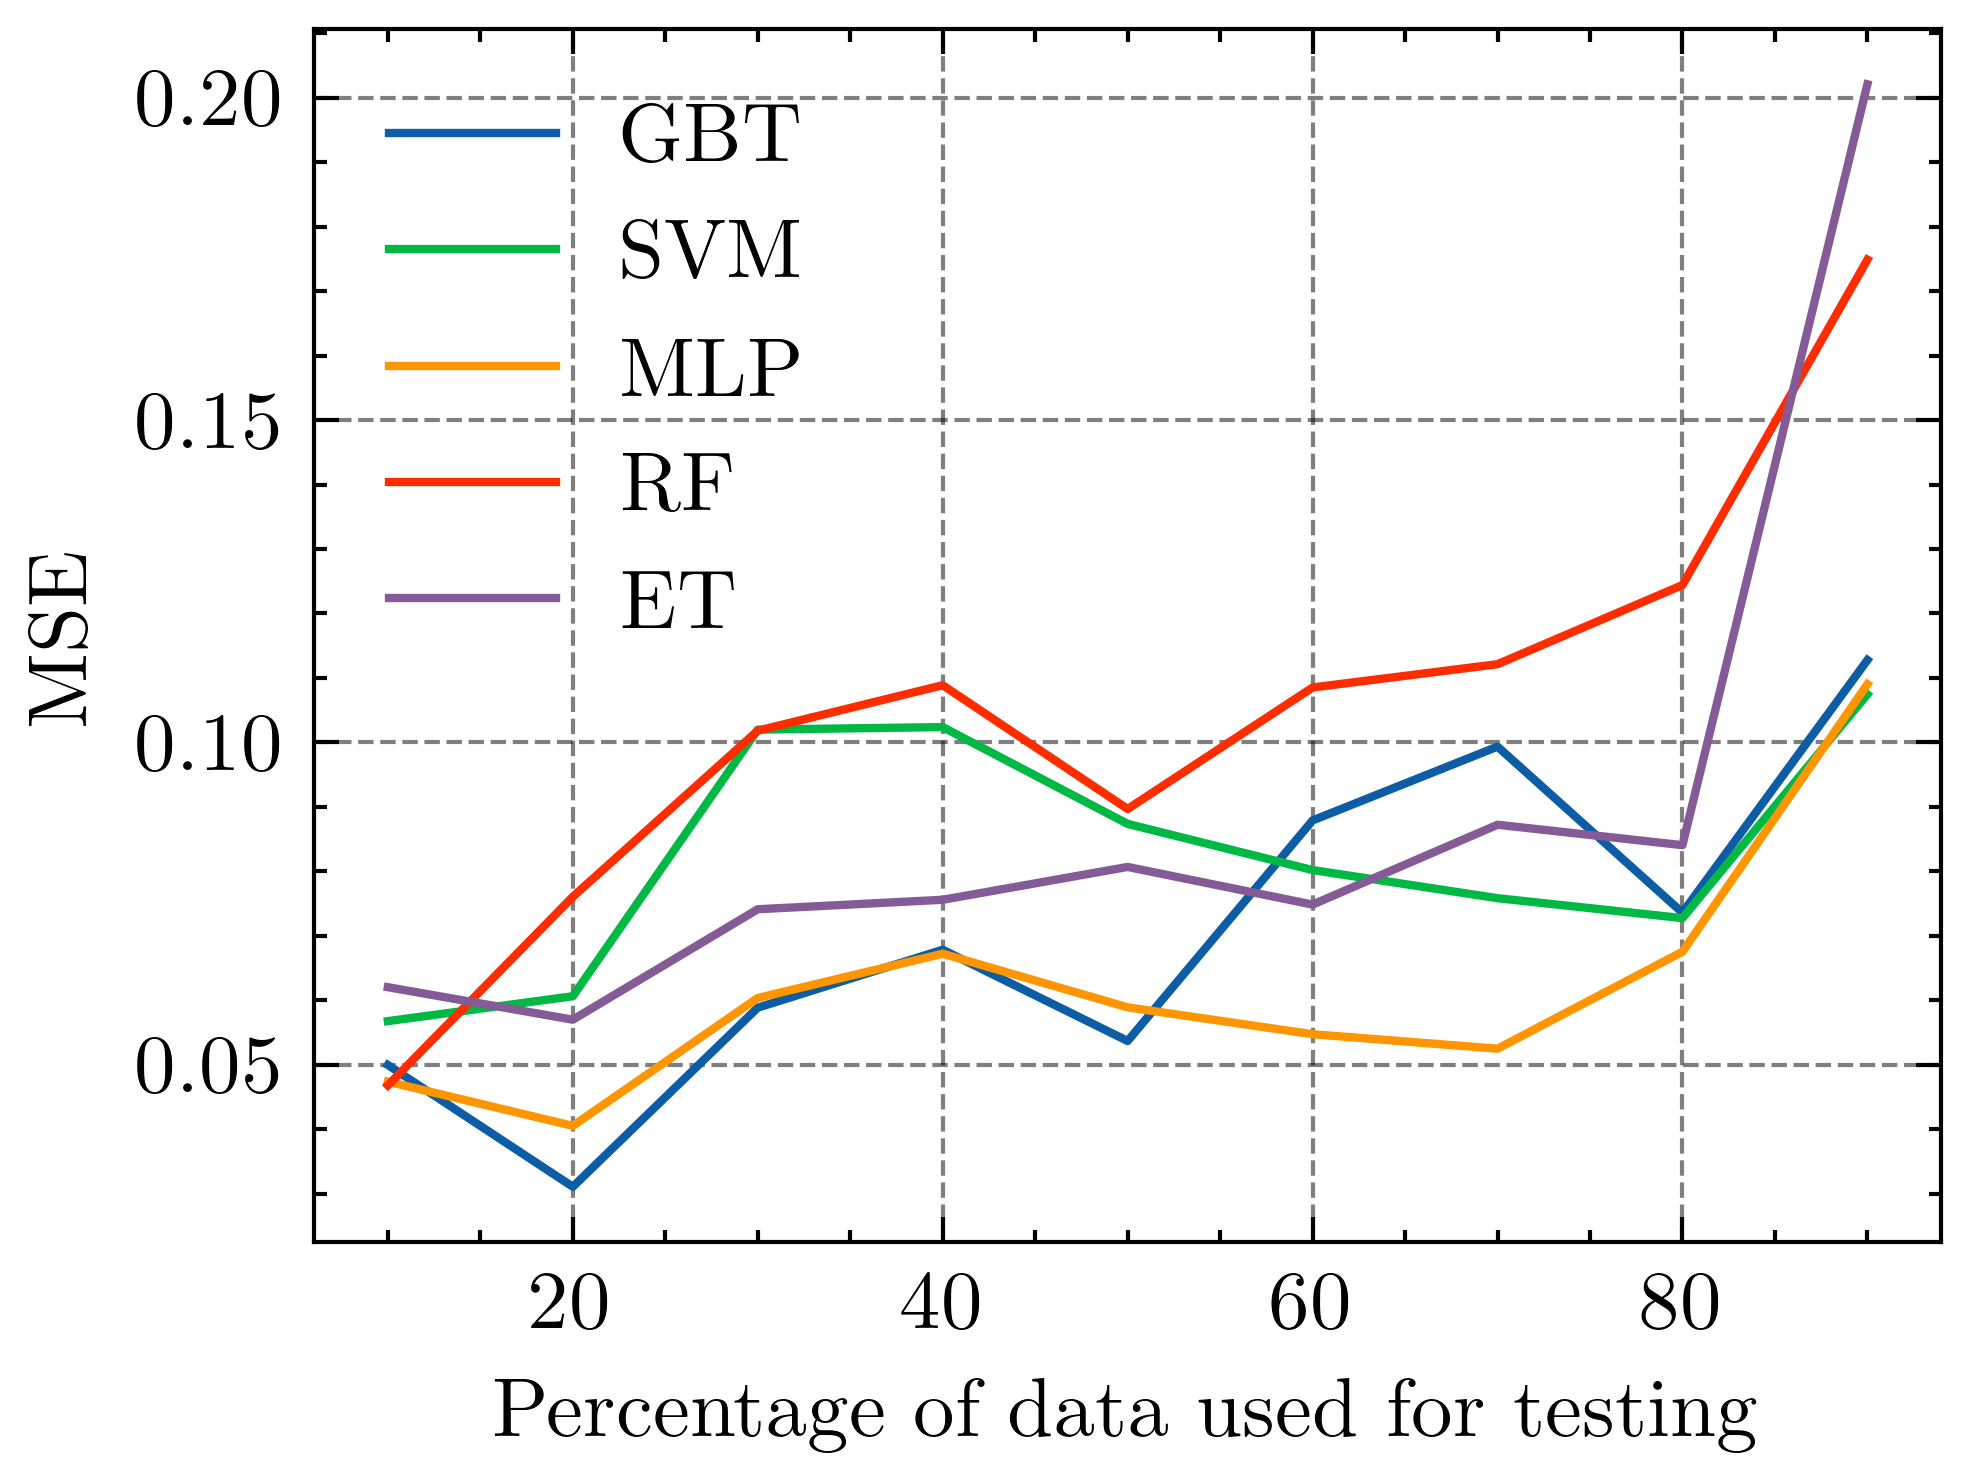
\includegraphics[width=\textwidth]{chap5/images/missing_values_plot}
            \caption{}
            \label{fig:first}
        \end{subfigure}
        \hfill
        \begin{subfigure}{0.4\textwidth}
            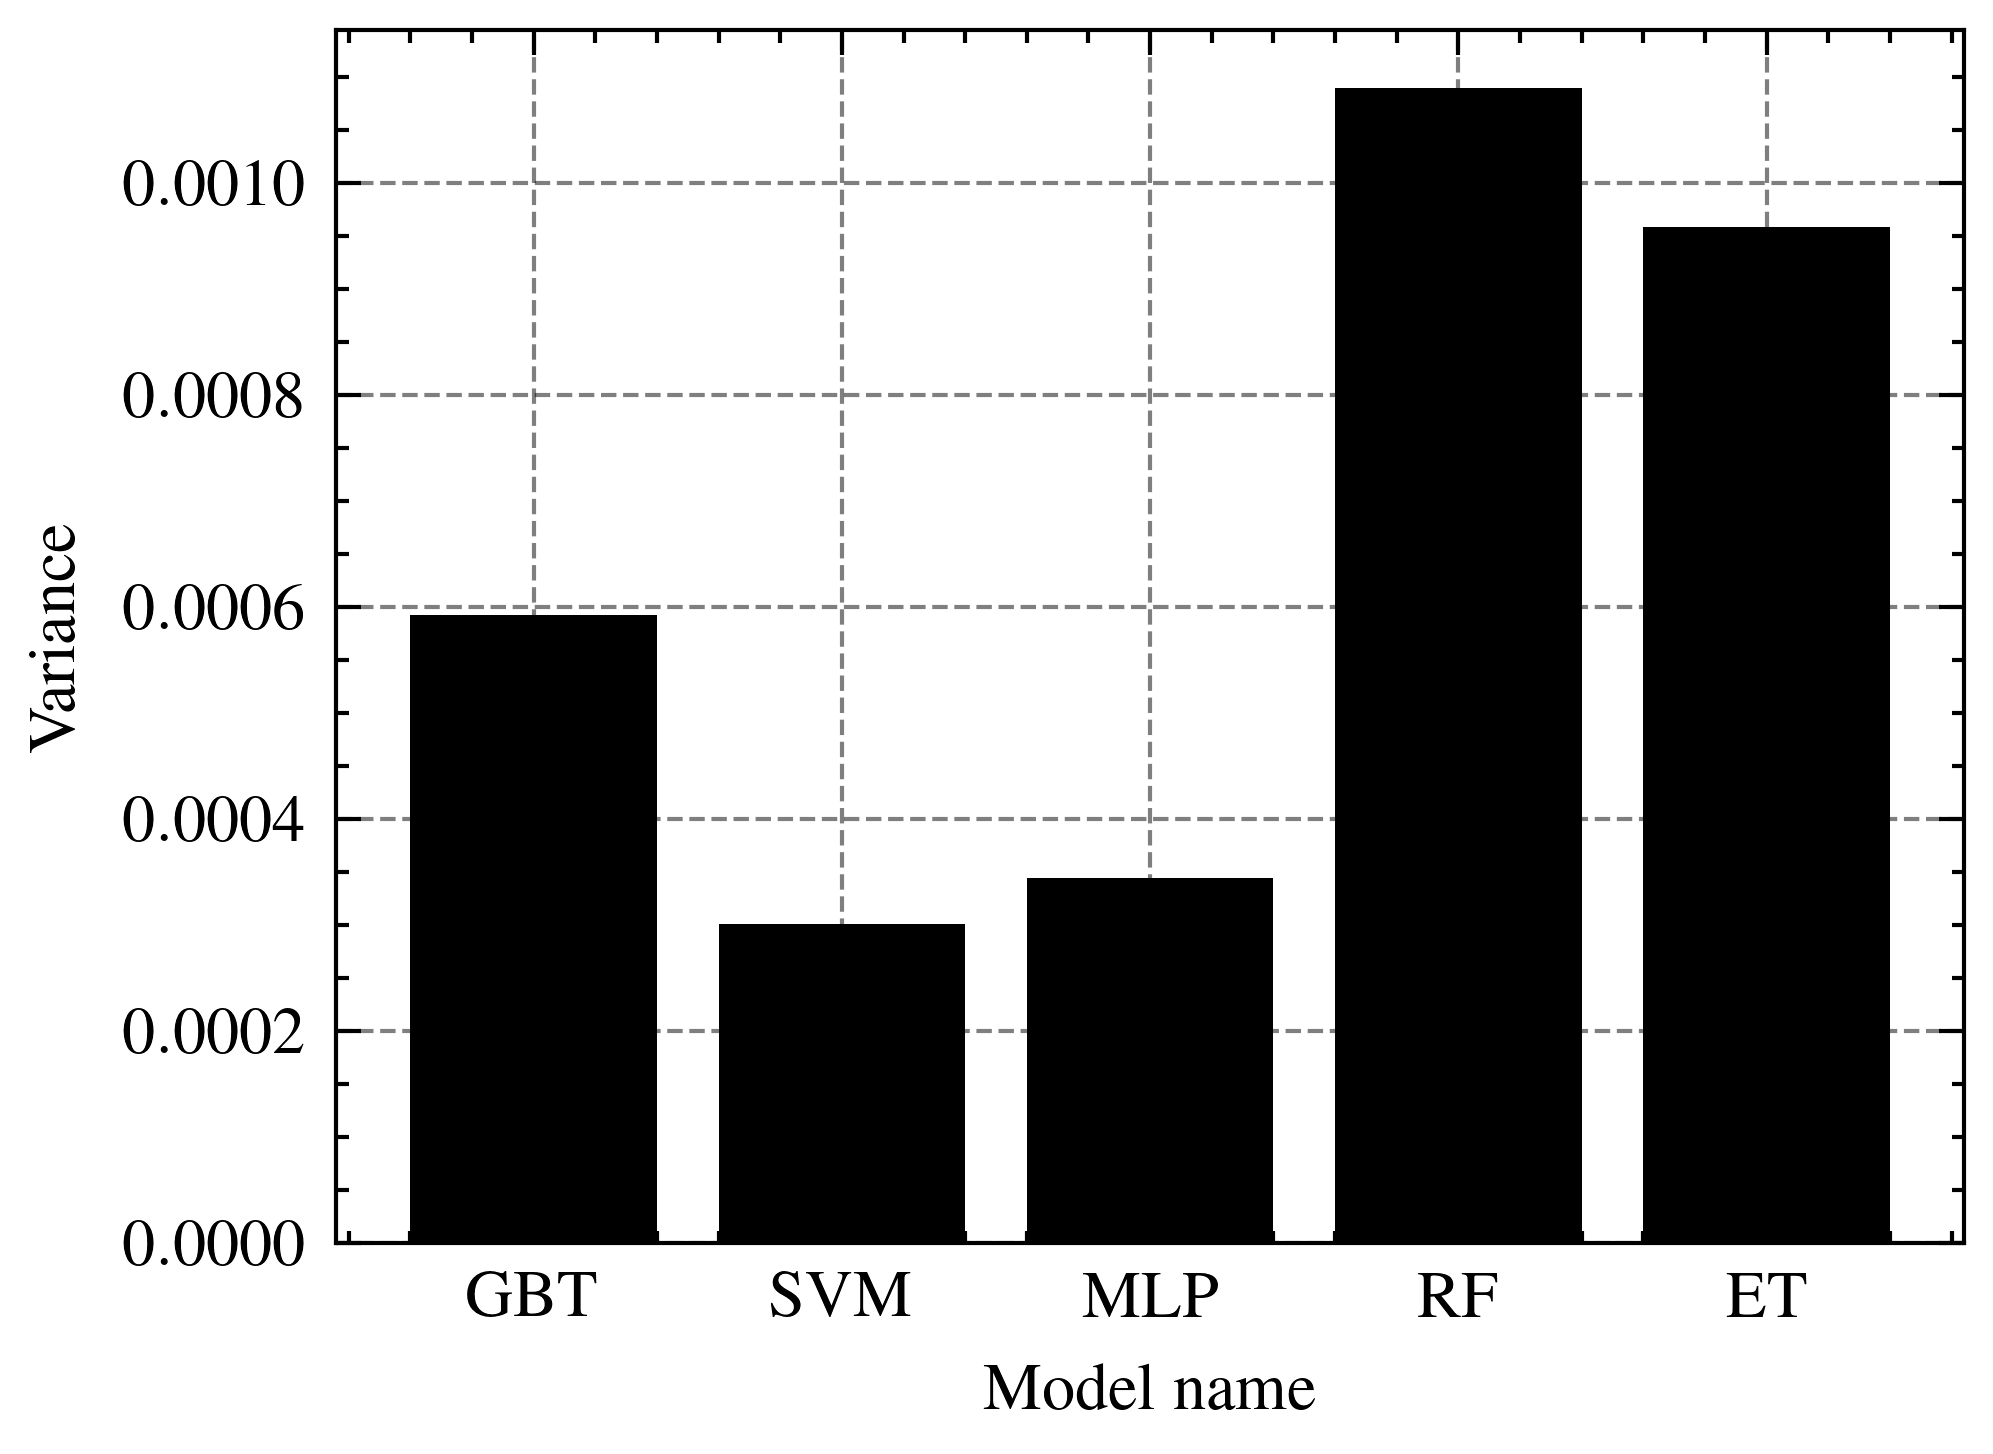
\includegraphics[width=\textwidth]{chap5/images/variance_missing_values}
            \caption{}
            \label{fig:second}
        \end{subfigure}
        \hfill
        \label{fig:results-missing-values}
    \end{tcolorbox}
    \caption{Figure (a) shows the comparison of performance on less data. Figure (b) shows the
    variance of the models when trained on less data.}
\end{figure}

%\begin{tcolorbox}[arc=0pt,boxrule=0.5pt]
%    \begin{equation}
%        \label{eq:average_loss}
%        \text{Loss of Accuracy} = \frac{1}{N} \sum_{i=1}^{N} |\text{RMSE}i -
%        \text{RMSE}{avg}|
%    \end{equation}
%\end{tcolorbox}

%Where \(N\) is the toal number of folds, \(i\) is the index of the current folds.
%
%It is worth noting that imputations of missing values can be used to mitigate
%the loss
%caused by missing data.
%However, this approach was not used in this thesis as the goal
%was to measure the robustness of the model to missing values specifically,
%rather than to
%artificially improve its performance through imputation techniques.

\subsection{Noise}\label{subsec:noise}
A common practise in \ac{ML} is to add noise to the training data to improve
the model's generalization abilities.
In the following section Gaussian Noise will be added to the data set to evaluate the robustness
of the model.

There is no standard approach to adding noise to the data.
In this thesis, the noise was added to the training data only.

To add the noise, \textit{numpy.random.normal} function was used, which
generate random numbers with a Gaussian distribution~\cite{scikit-learn}.
The mean and standard deviation of each feature were calculated based on the
original data, and the function was used to generate noisy values for each feature.

To study the model's reaction to increasing amounts of noise, the noise added
to the training data was gradually increased starting from 1\% to 50\%, which means that the
last iteration contains as many noisy as ``clean'' samples.

The difference between all \ac{RMSE} between iterations was defined as loss.
The total loss was calculated by averaging the difference of these values as shown in Equation~\ref{eq:noise}.

\begin{tcolorbox}[arc=0pt,boxrule=0.5pt]
    \begin{equation}
        \text{Average Loss} = \frac{1}{N} \sum_{i=1}^{N} |\text{RMSE}i -
        \text{RMSE}{avg}|\label
        {eq:noise}
    \end{equation}
\end{tcolorbox}

\begin{itemize}
    \item \textit{Does the calculation of the loss make sense?}
\end{itemize}

\subsection{Results}\label{subsec:results-robustness}

\begin{table}[H]
    \begin{tcolorbox}[arc=0pt,boxrule=0.5pt]
% \sisetup{group-minimum-digits = 4}
        \centering
        \begin{tabular}{llll}
            \toprule
            \thead{\textbf{Model Name}} & rs & {\thead{\textbf{Noise} \\ \unit{loa}}}
            \\
            \toprule
            \textbf{LR} & - & 0.070 & 0.251 \\
            .071 & 0.224 \\
            \hdashline
            \textbf{Random Forest} & x & 0.241 \\
            \hdashline
            \textbf{SVM} & - & 0.251 \\
            \hdashline
            \textbf{MLP} & - & 0.451 \\
            \bottomrule
        \end{tabular}
        \caption{Results of used machine learning models regarding the design
        principle robustness.}
        \label{tab:results_robustness}
    \end{tcolorbox}
\end{table}


\section{DP4: Stability}\label{sec:stability}
% Does the artifact generate repeatable results when trained on different data?
% Leave-one-out cross-validation stability 
Stability is defined as the ability of the model to generate repeatable
results when trained on different data~\cite[p. 16]{siebert2022construction}.

One appropriate way to measure the stability of a model is to use \ac{LOOCV},
which is a a form of \ac{CV} where one sample is used for validation and the remaining
data is used for training~\cite[p. 200--201]{gareth2013introduction}.
LOOCV is a technique where the observation set is divided into two parts, but instead of having
two subsets of comparable size, one sample is used for validation, while the rest form the
training set.

In order to evaluate the model the \ac{LOOCV} was repeated for all samples in
the dataset resulting in a total of \(n\) iterations.
The stability of the model was determined by calculating the average prediction error across all
iterations, using the equation provided in Equation~\ref{eq:loocv} which is taken from~\cite[p.
201]{gareth2013introduction}.

\begin{tcolorbox}[arc=0pt,boxrule=0.5pt]
    \begin{equation}
        CV_{(n)} = \frac{1}{n} \sum_{i=1}^{n} \text{MSE}_{i}\label{eq:loocv}
    \end{equation}
\end{tcolorbox}

The resulting \ac{MSE} is a poor estimate of the model's generalization error because only one
sample is used for validation~\cite[p. 201]{gareth2013introduction}, but it can be used to make a
statement about the stability.

The stability of the model can be evaluated by examining the standard derivation of the cross
validations scores.
A low standard derivation across all folds indicated that the model can generated consitent
results when trained on different datasets, suggesting are more sable model.

It is important to note that there are many different ways to measure the modelstability.
In this work LOOCV was chosen for three reasons.
%Another common approach is to use regular Cross-Validatoin, there are three reasons why LOOCV was
%chosen for this work.
Firstly, \ac{LOOCV} uses nearly all available data for training, while K-fold CV resevers a
portion o f the data for testing.
as the dataset used is relatfively small, it is an advantage to use all data for training.
Secondly, \ac{LOOCV} tends to have a lower bias due to the larger training set.
Lastly, multiple approaches have been tried to measure the model stabilty, and LOOCV delivered
he most stable and interpretable results.
The main drawback of the chose method is that it is computationally expensive as it required n
iterations.

Table~\ref{subsec:results-stability} shows the cross-validation score and the standard derivation
of each model. The focus relied more on the standard derivation, as it is a better indicator of
the stability of the model. As already mentioned the \ac{CV} score with using LOOCV is a poor
estimator.

---

\subsection{Results}\label{subsec:results-stability}

\begin{table}[H]
    \begin{tcolorbox}[arc=0pt,boxrule=0.5pt]
% \sisetup{group-minimum-digits = 4}
        \centering
        \begin{tabular}{ll}
            \toprule
            \thead{\textbf{Model Name}} & \thead{\textbf{std of CV scores (MSE)}}
            \\
            \toprule
            \textbf{Random Forest}          & 0.047 (0.891) \\
            \textbf{Random Forest}          & 0.200 (0.047) \\
            \hdashline
            \textbf{Gradient Boosting}      & 0.044 (0.922) \\
            \textbf{Gradient Boosting}      & 0.190 (0.039) \\
            \hdashline
            \textbf{Extra Trees}            & 0.46  (0.877)   \\
            \textbf{Extra Trees}            & 0.199 (0.053) \\
            \hdashline
            \textbf{Support Vector Machine} & 0.050 (0.853) \\
            \textbf{Support Vector Machine} & 0.266 (0.061) \\
            \hdashline
            \bottomrule
        \end{tabular}
    \end{tcolorbox}
    \caption{Results of the stability of the models.}
    \label{tab:results-stability}
\end{table}


\section{DP5: Resource utilization}\label{sec:resource-utilization}
% How much resources are required to train and run the model?
% Training time, runtime, storage space

To measure the resource utilization of the model, the following metrics are
used:

% From Copilot
\paragraph*{Training time}
Measured in seconds. Refers to the time it takes to train the model.
Training a model requires resources such as memory, CPU, and GPU, therefore
the longer it takes
to train a model, the more resources are required. According to resources
utilization a shorter
training time is desirable.

The training time is measured using the \texttt{time.time} function in python
. The function
returns the time in seconds since the epoch. The time is measured before and
after the model is
fitted. The difference between the two times is the training time.

\textbf{Inference time}
Measured in milliseconds. It refers to the time it takes to make a prediction
on data once it has
been trained.
It is an important measure not only for real-world application but also a
faster runtime uses
less resources and is therefore more efficient.

\textbf{Inference time}
Measured in milliseconds. Time it takes to make 100 predictions.
A model that takes longer to make predictions may be more complex than a
model that is able to
make predictions more quickly.
Measured using the \texttt{time.time} function in python. 100 valuees are
picked out of the teset
set and the time is measured before and after the prediciton is made.

\textbf{Memory space}
Measured in Mb.
It refers to the amount of memeory required to run the model.
The more storage space required to store the model, the more resources are
required to store it.
Therefore, a smaller storage space is desirable.
To measure the memory usage the \texttt{memory\_usage} function from the
\texttt{memory\_profiler}
package is used.


\begin{table}[H]
    \begin{tcolorbox}[arc=0pt,boxrule=0.5pt]
        \centering
        \begin{tabular}{llll}
            \toprule
            \thead{\textbf{Model Name}} & {\thead{\textbf{
                Training
                time} \\
            \unit[]{ms}}}
            & {\thead{\textbf{Inference time} \\ \unit[]{ms}}} &
                {\thead{\textbf{Memory
            Usage} \\
            \unit{kb}}}
            \\
            \toprule
            \textbf{DT}  & 2.743    & 1.136  & 174.0 \\
            \hdashline
            \textbf{RF}  & 25.205     & 2.886  & 173.219 \\
            \hdashline
            \textbf{ET} & 19.62    & 1.725  & 173.121 \\
            \hdashline
            \textbf{GBR} & 46.302   & 1.343  & 158.125 \\
            \hdashline
            \textbf{SVM} & 309.721 & 2.789 & 195.734 \\
            \hdashline
            \textbf{MLP} & 19100.697 & 11.663 & 180.949 \\
            \bottomrule
        \end{tabular}
        \caption{Overview of the used machine learning models and their metrics.}
        \label{tab:resutls_resource_utilization}
    \end{tcolorbox}
\end{table}

As can be seen in Table~\ref{tab:resutls_resource_utilization}, the \ac{ET} is faster
than to th conventional \ac{RF}.
This expected since the most-time intensive part of the \ac{RF} is the splitting of the
nodes with determining the optimal threshold for each feature at each node
(see section~\ref{subsubsec:extra-trees}).
It has been observed, that this advantage is lost when the \texttt{n\_estimators}
parameter is set above 10.

The \ac{GBR}  does use less memory than the \ac{RF} and \ac{ET}, because it heavily prunes the generated trees, in
the trained model the \texttt{max\_depth} parameter is set to 5.
This results in a shorter inference time and a bit less memory space compared to the other tree based models.

The \ac{MLP} is the slowest model to train and to make predictions.
Most certainly this is because an \ac{MLP} typically has more parameters to learn and
has a deeper architecture, which means that it requires mor computations to train and
predict.
Also the training algorithm used is backpropagation, wich can be more computationally
intensive.
Also an \ac{MLP} trains all data at once and therefore cant parallelize the process.
It has to be noted, that tuning the hyperparameters is a time-consuming steps and the
chosen parameters might not be the optimal ones.


\section{DP6: Interpretability}\label{sec:interpretability}
% How well can the model be explained?
% Complexity measures (e.g., no. of parameters, depth)

% Sieber et al used
% %
%& Complexity measures (e.g., no. of parameters, depth) \\
% These metrics where changed
When following definitions of interpretability used in
section~\ref{sec:objectives-of-a-solution}, it is clear that it is not possible to
measure interpretability in a quantitative way, but other metohds can beu sed to measure the
interpretability of a model.
%Interpretable models allow the usage of global model-agnostic evaluation
%methods which will be used later in the evaluation of the models (see
%Section~\ref{sec:evaluation}).


According to~\cite{molnar2020interpretable} one way to make a model interpretable is to limit the
choice of algorithms to those that produce interpretable results.
Example of such algorithms include linear regression, logistic regression and decision
trees~\cite[p. 35]{molnar2020interpretable}.

%\cite{molnar2020interpretable} defines three properties of interpretable models: linearity,
%monotonicity and interactions.
%A linear model expresses the relationship between features and the target outcome aa a linerar
%equation~\cite[]{molnar2020interpretable}.
%Monotonocitiy constraints ensure that there is a consistent relationship between a feature and
%the target outcome across the etnire renage of the feature. This can make it easier to understand
%the relationship.
%Some models automatically include interactions between features to improve prediciotn, while
%other require the manual creation of interaction features. However, inlcuding too many or complex
%interactions can make the model more difficult to interpret~\cite{molnar2020interpretable}.

%In the model selection for this thesis the focuses mostly on interpretable models,
%as they are easier to understand and explain, therefore mostly models are chosen which fulfill
%all three properties.
%
%Later in the thesis, the interpretability of the models is used to explain
%the results.

\subsection{Interpretable Models}\label{subsec:interpretable-models}
Linear Regression and Decision Trees are considered as interpretable models and offer good
model-specific explanations by default~\cite{molnar2020interpretable}.
As mentioned in section~\ref{sec:dp1:-correctness}, both algorithms perform not good enough
to be considered as a solution for the problem.
Therefore the focus is on model agnostic methods to explain the predictions of the models.

Also~\cite{molnar2020interpretable} differentiates between global and local
interpretability. Global
interpretability refers to the ability to understand the overall behavior of
the model, while local interpretability refers to the ability to understand the behavior of the
model for a specific instance.

As seen in the previous sections six different models were trained.
It does not make sense to apply model-agnostic method on all six models, it makes more sense to
apply the methods on the best performing models.

Therefore in a first step in the section~\ref{subsec:overall-comparison-model-performance} the
best performing models
are identified and in a second step model-agnostic interpretability methods are applied to
explain the predictions of the models.

For the current dataset, the V/t ratios range from 3.3 to 100. The highest ratio can be achieved
by bending a 0.5 mm thin metal sheet using a 50 mm wide die opening, while the lowest ratio is
achieved by bending a 3 mm thick sheet on the same die opening.

Recommended V/t ratios in industrial practices are between 6 and 10~\cite[p.7]{
    cruz_applicationmachinelearning_2021}.
Bending operations performed outside of this range of recommended ratios may result in
high spring back.

The selected representative instances for the local methods are from one of three cases:
\begin{itemize}
    \item Case A includes instances with V/t ratios below the recommended range.
    \item Case B includes instances within the recommended range of V/t ratios.
    \item Case C includes instances with V/t ratios above the recommended range.
\end{itemize}

Chosen instances from each case are shown in Table~\ref{tab:representative-instances}.

\begin{table}[H]
    \begin{tcolorbox}[arc=0pt,boxrule=0.5pt]
        \centering
        \begin{tabular}{lllll}
            \toprule
            \textbf{Case} & \textbf{\(V\) } & \textbf{\(t\)} & \textbf{\(y_p\)} & \textbf{V/t} \\
            \toprule
%            A             & 10              & 2.0            & ?                & 5            \\
            A             & 20              & 3              & ?                & 6.66         \\
            \hdashline
            \hdashline
            B             & 30              & 2              & ?                & 15           \\
            B             & 20              & 1              & ?                & 20           \\
%            B             & 30              & 1.5            & ?                & 20           \\
            \hdashline
            C             & 50              & 1              & ?                & 50           \\
            C             & 50              & 0.5            & ?                & 100          \\
            \bottomrule
        \end{tabular}
    \end{tcolorbox}
    \caption{Representative instances for the local methods.}
    \label{tab:representative-instances}
\end{table}



\subsection*{Global Model-Agnostic Methods}
In the following section global-model-agnostic methods are are applied to the trained machine
learning models in order to understand the overall behavior of the models.

There are two commonly used methods for analyzing the relationship between input features and the
target variable: feature dependence plots and partial dependence plots.
In the case of \ac{MLP} has no built-in feature importance, because the importance of each
feature is determined by the weights assigned to the perceptron.
The \ac{SVM} the feature importance cannot be directly derived from the model beacuse the
algorithms applies a hyperplane that separates the data.
The importance of the feature depeneds on the influence of the hyperplane and that is not easily
measurable.
Therefore not feature importance can be plotted for the two chosen models. Other models like the
random forest have a built-in feature importance, which can be used to analyze the model.

Figure~\ref{fig:feature_impoartances_rf} compares and visualizes the relative
importance of the features used for training the model.
As shown, the thickness is the most important feature followed by distance
and die opening.
The results shows, that all three featured are relevant for the outcome and so no feature can be
removed from the dataset to get a better performance of the model.

\begin{figure}[H]
    \begin{tcolorbox}[arc=0pt,boxrule=0.5pt]
        \centering
        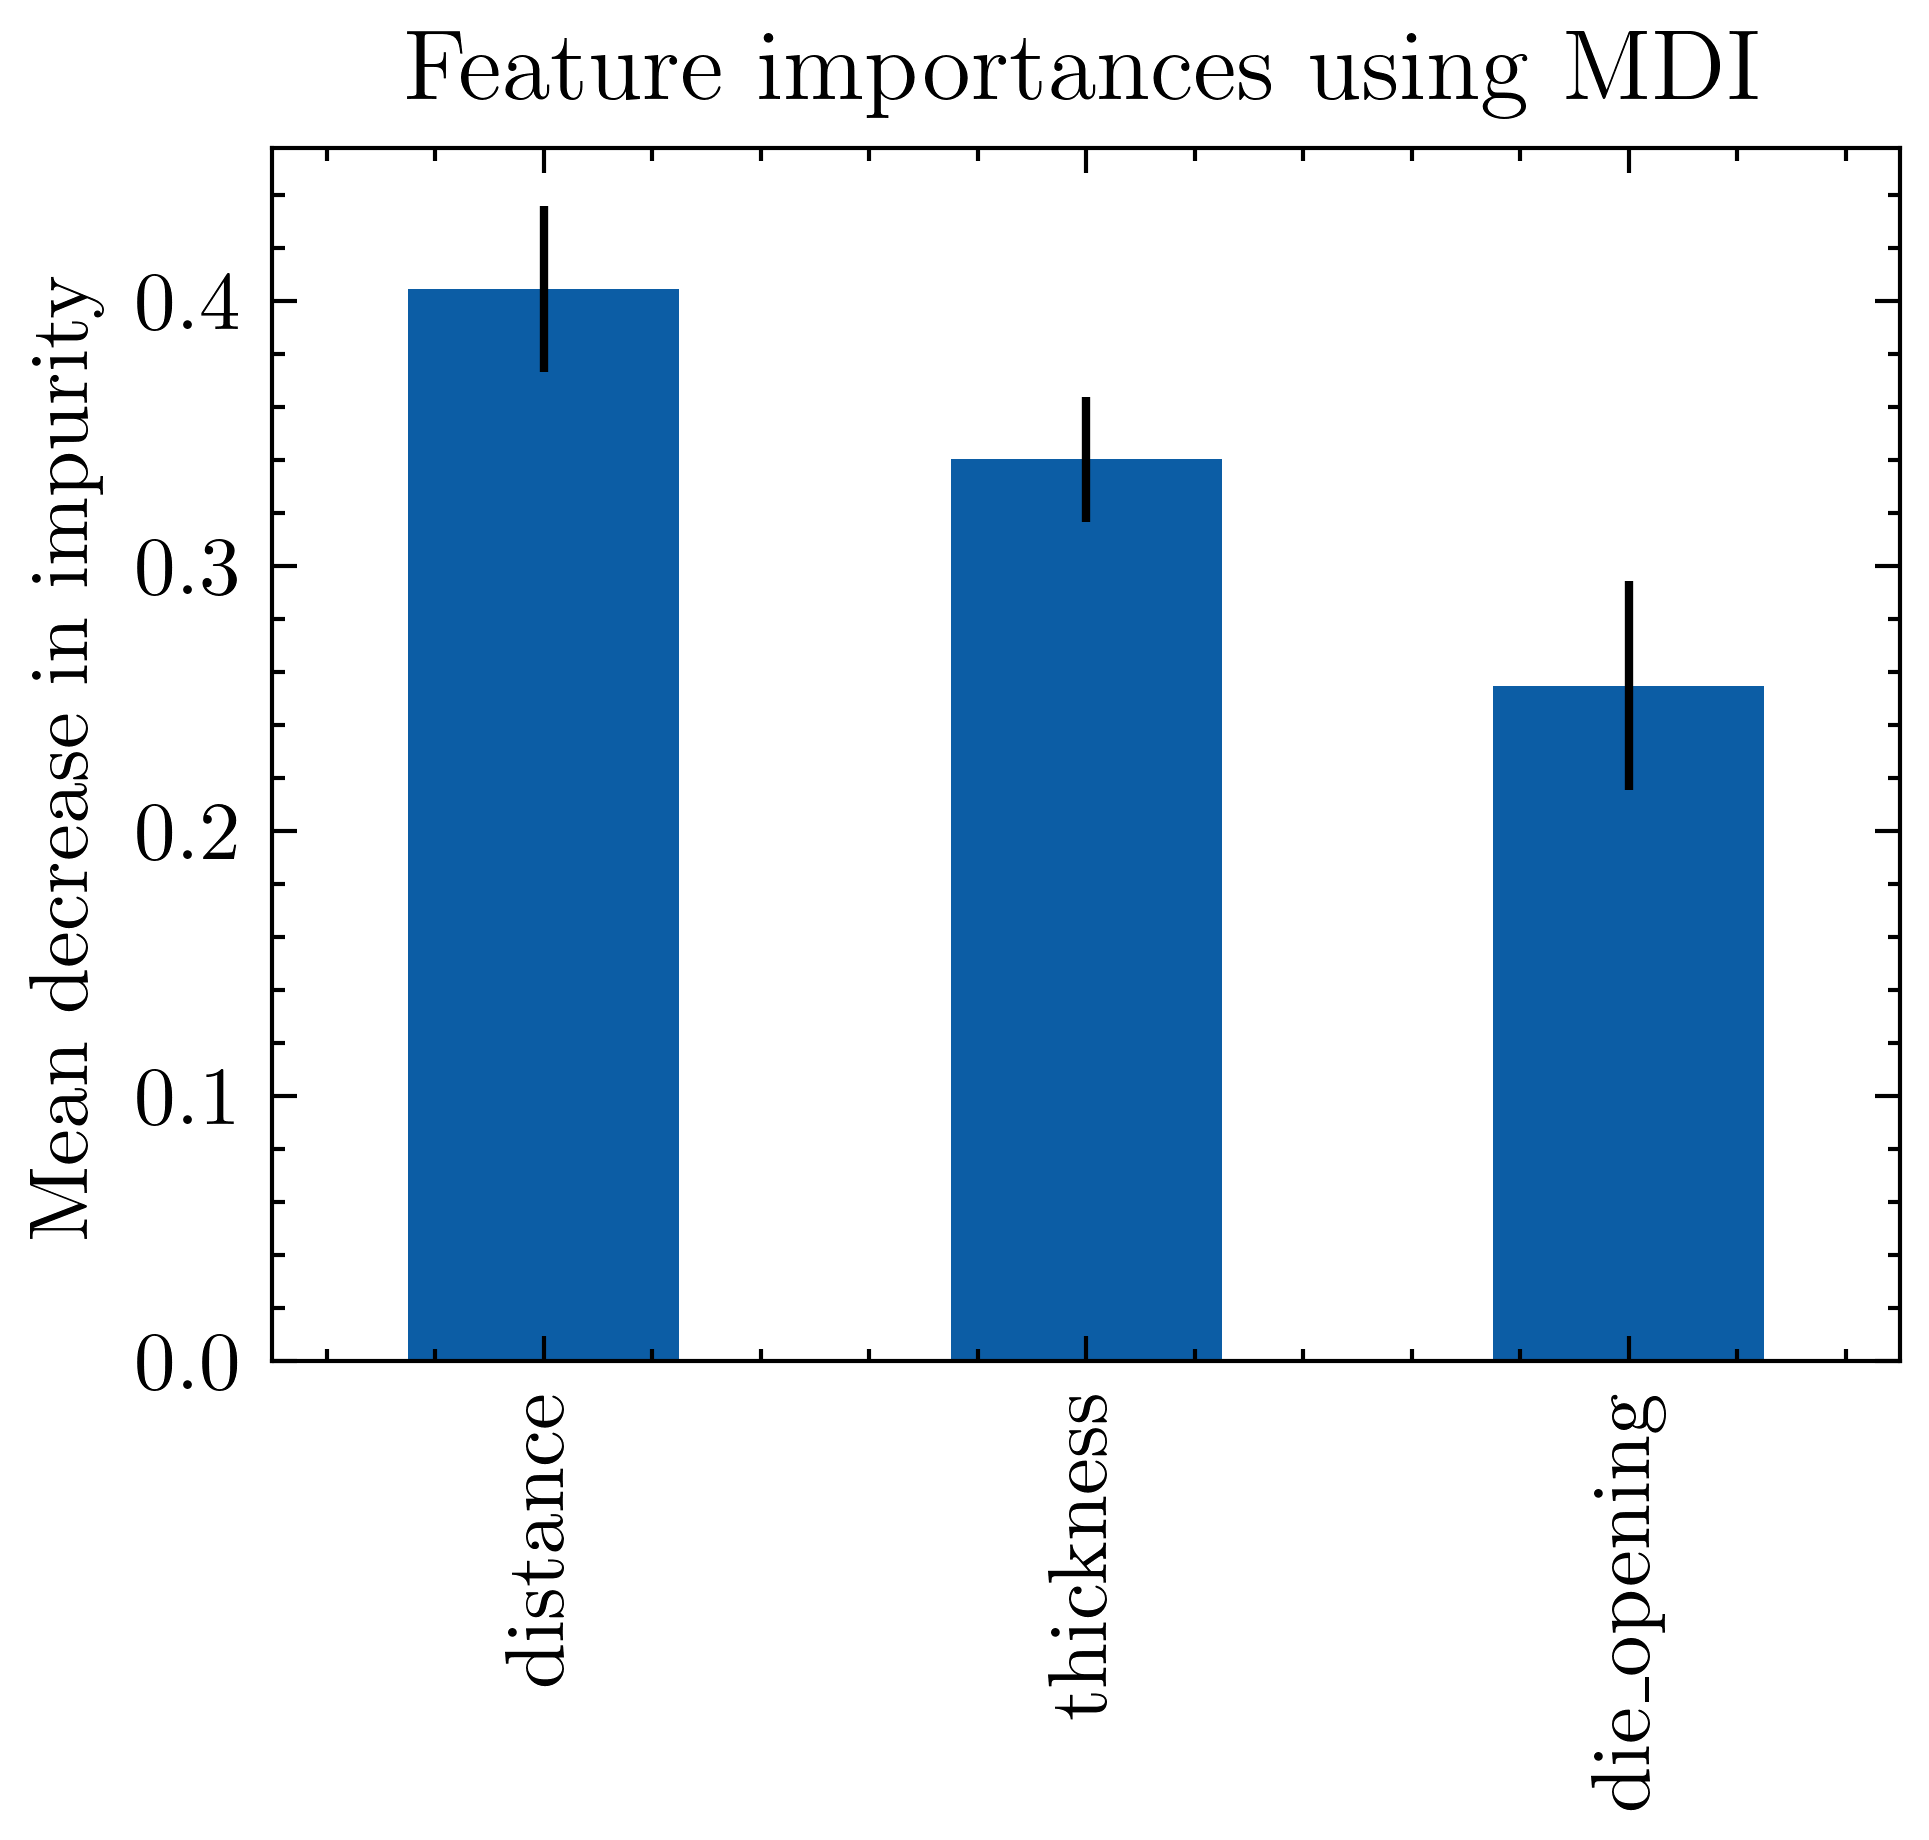
\includegraphics[width=0.9\textwidth]{chap5/images/rf_feature_importances}
    \end{tcolorbox}
    \caption{Feature importance of the random forest model.}
    \label{fig:feature-importances-rf}
\end{figure}

\subsubsection{Partial Dependence}
Feature dependence plots illustrate the relationship between a feature and the target variable.
By analyzing these plots, we can identify which features have the strongest impact on the model's
predictions, making it easier to prioritize and refine our feature selection.

Partial dependence plots, on the other hand, examine the impact of a single input feature on the
target variable while keeping all other features constant.
These plots can help us understand which individual features have the most significant impact on
the target, enabling us to fine-tune our feature engineering and gain deeper insights into the
underlying relationships in our data.

Both of these methods are powerful tools for understanding the role of input features in
predictive modeling, and can be used together to gain a comprehensive understanding of the
factors that drive model performance.

\cite{greenwell2018simple} introduced a another feature importance measure based on partial
dependence.
Partial dependence refers to the relationship between a target variable and a single predictor
variable in a statistical model, while keeping all other predictor variables constant.
A feature that has a consistent partial dependence across all values is less important than a
feature that exhibits significant variations~\cite[p. 117--118]{molnar2020interpretable}.


Figure~\ref{fig:partial_dependence_plots}, we can see the PDPs for two models: Support Vector
Machines (SVM) and Multilayer Perceptron (MLP).
The results show that a higher \(y_p\) value leads to a greater spring back, while increasing the
thickness of the metal sheet results in a lower spring back.
The effect of the die opening is less significant than the other two features, but there is still
a noticeable increase in spring
back with higher die opening.

The PDPs demonstrate that all features exhibit a non-linear relationship with the target variable.
This information can be useful for understanding the behavior of the models and the impact of
different features on the predicted outcome.

\begin{figure}
    \begin{tcolorbox}[arc=0pt,boxrule=0.5pt]
        \centering
        \begin{subfigure}{0.45\textwidth}
            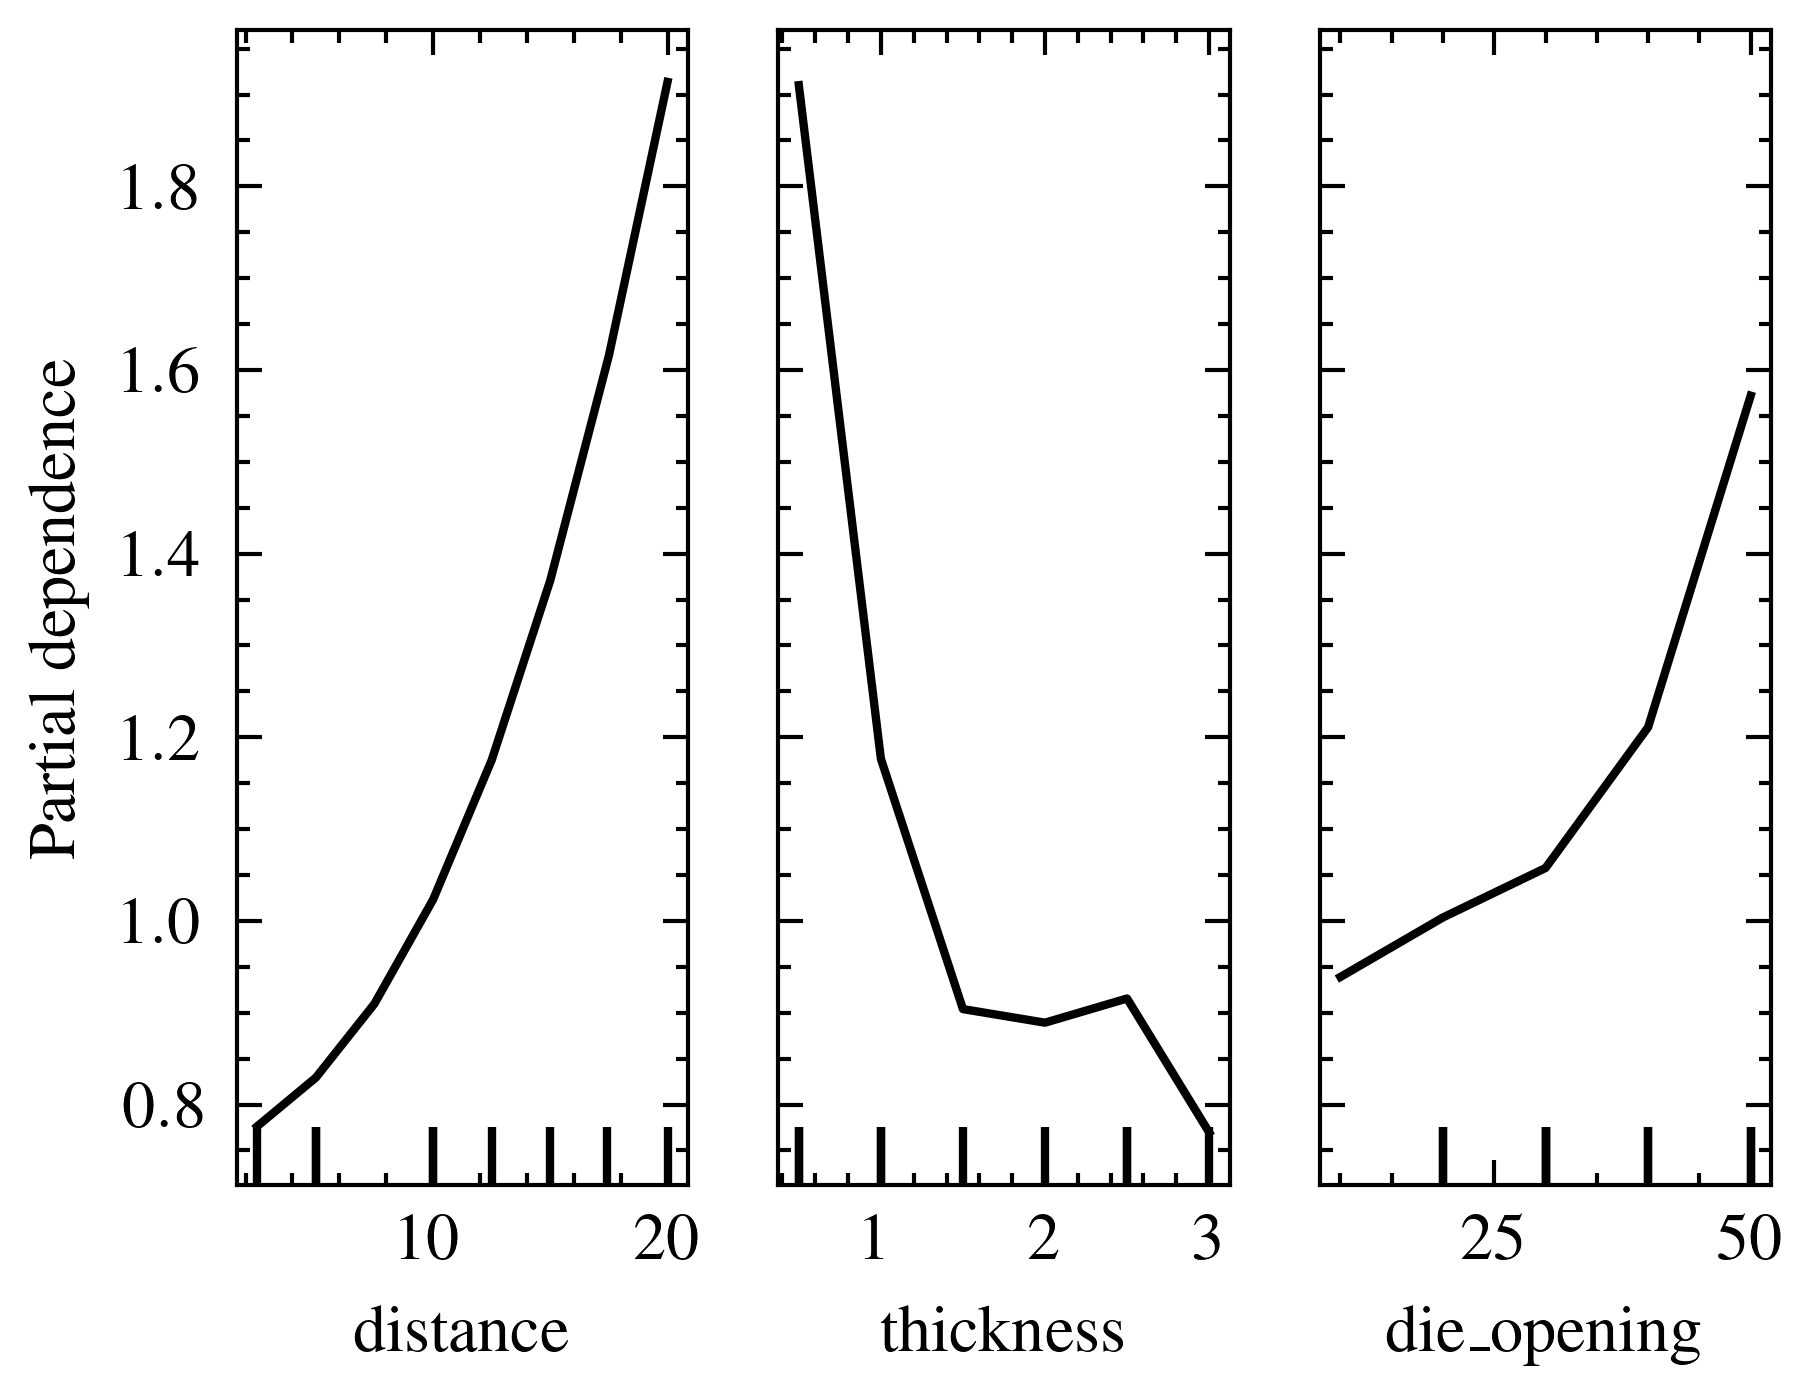
\includegraphics[width=\textwidth]{chap5/images/partial_dependence_SVM}
            \caption{SVM}
            \label{fig:feature_impoartances_rf}
        \end{subfigure}
        \hfill
        \begin{subfigure}{0.45\textwidth}
            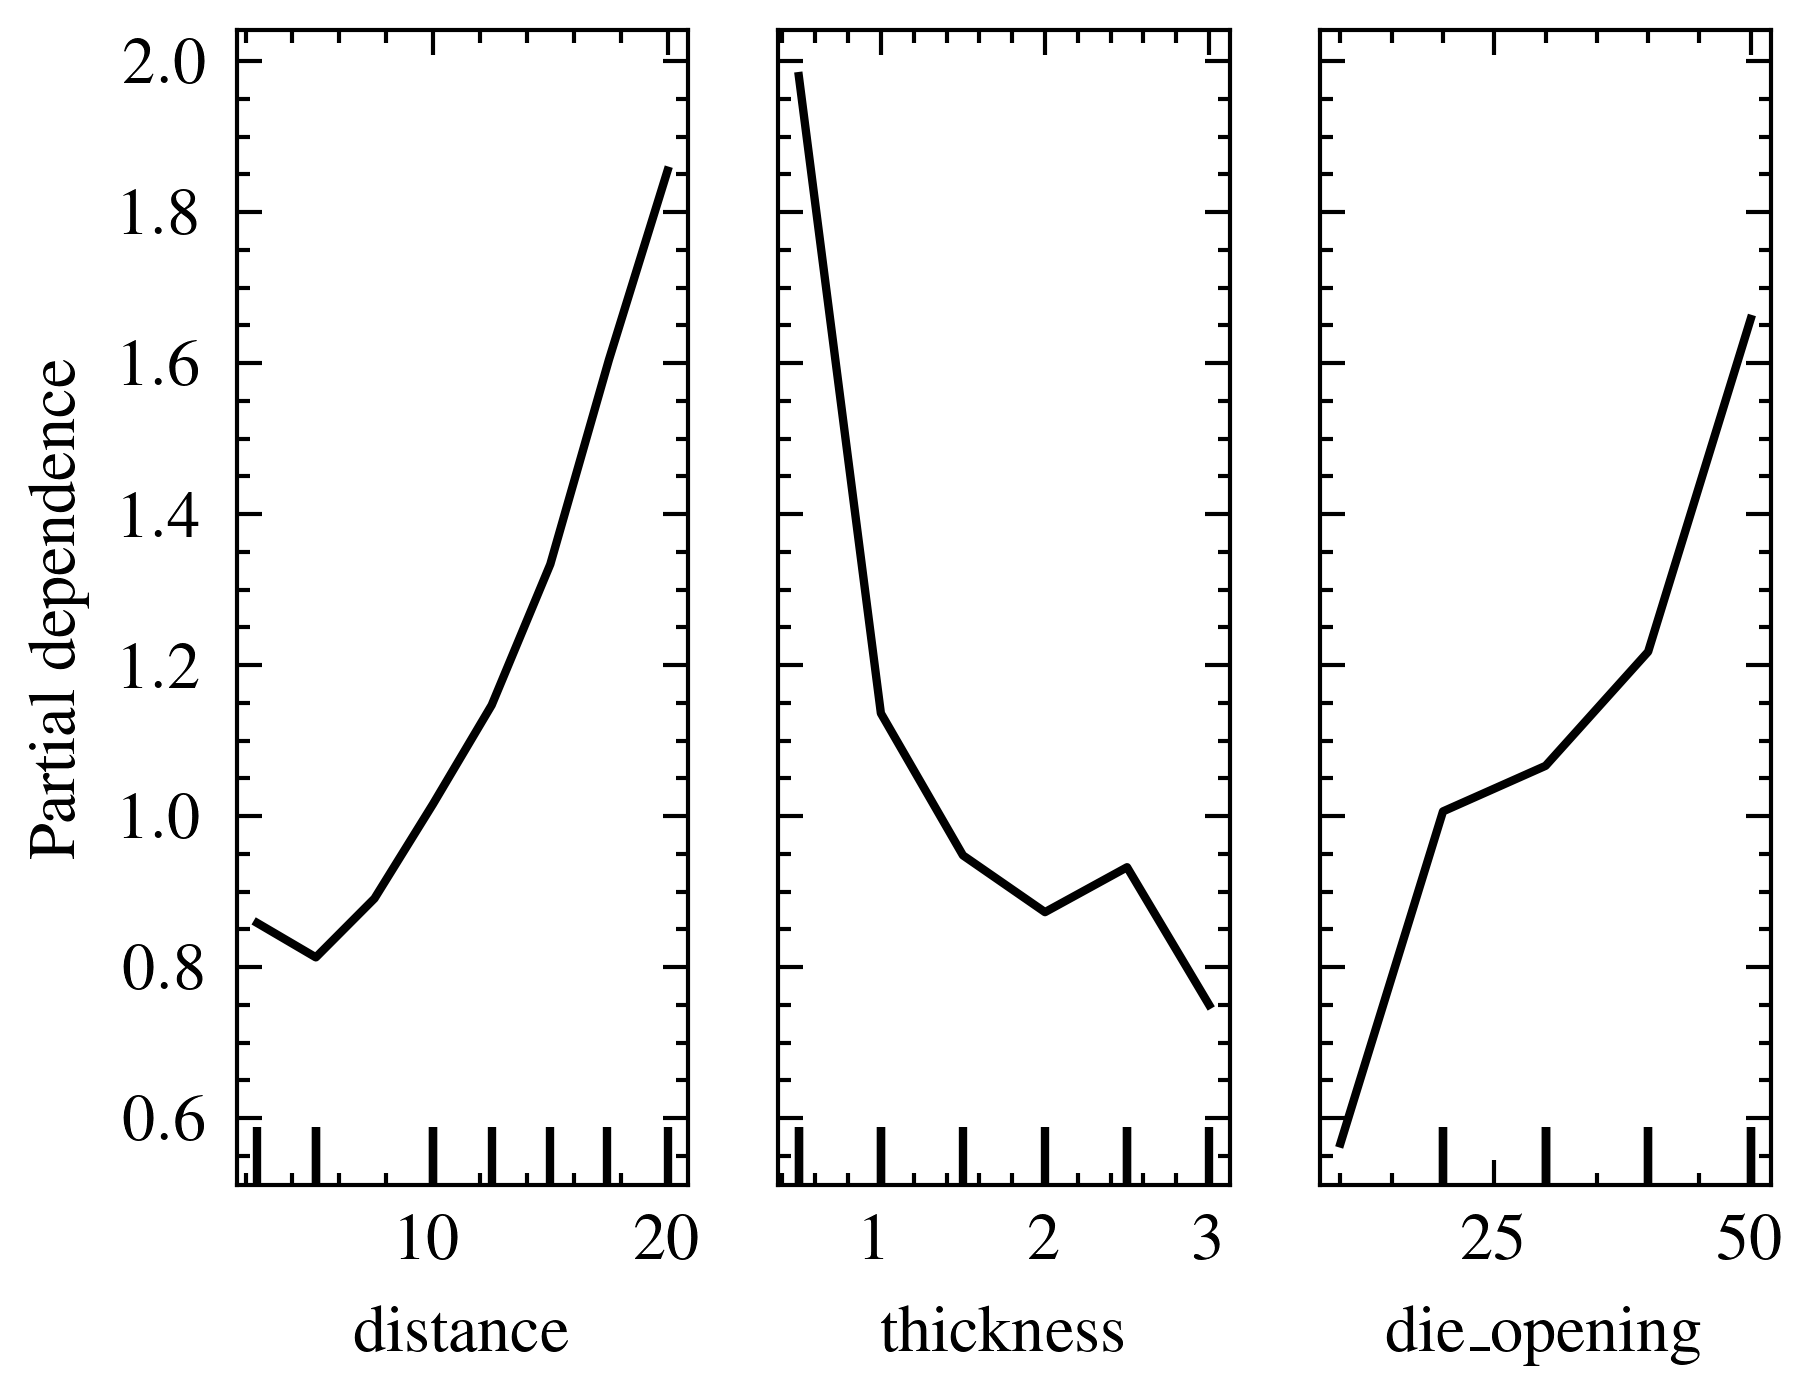
\includegraphics[width=\textwidth]{chap5/images/partial_dependence_MLP}
            \caption{MLP}
            \label{fig:partial_dependence_svm}
        \end{subfigure}
        \hfill
        \caption{Partial dependence plots}

        \label{fig:partial_dependence_plots}
    \end{tcolorbox}
\end{figure}

It is important to note that partial dependence plots and feature importance plots are limited to
identifying linear relationships between features and the target variable.
Since this is not the case as state previously, the results of the partial dependence plots are
alternative models as permutation feature importance and SHAP values are used to gain further
information.

\subsection{Permutation Feature Importance and SHAP}\label{subsec:permutation-feature-importance-
and-shap}

Permutation feature importance's asseses the impact on the model's prediction error when the values
of a feature a randomly permutes. Permutation in this context means the proces of randomly
shuffling the values of a single features while keeping the values of all other feautres unchanged.
Thereby the association between the feature and the actual outcome is disrupted~\cite[p. 157]{
    molnar2020interpretable}.

The importance of a feature is evaluated by assessing the degree to which permuting its values
results in an increase in the prediction error fo the model.
If permuting a features results in a significant increases in errors the features is deemed
important because the model relied on it for making accurate predictions.
Conversely, if permuting a feature doesn't change the prediction error is considered unimportant
because the model didn't utilize it for it's prediction~\cite[p. 158]{molnar2020interpretable}.

Figure~\ref{fig:permutation_feature_importance} shows the permutation feature importance for the
\ac{MLP} and \ac{SVM} models.
Interestingly, the results show that the permutation feature importances for the die opening is
always zero.
This could mean that the die opening is not relevant for the overall decision making of both
models.
The normal feature importance plots showed that die die opening is important so that might not be
explanation.
So most likely the die opening is still and important feature when combined with either the
thickness ore the penetration distance.




\begin{table}[ht]
    \begin{tcolorbox}[arc=0pt,boxrule=0.5pt]
        \centering
        \subfloat[Subtable 1 list of tables text][MLP]{
            \begin{tabular}{lll}
                \toprule
                \multicolumn{3}{}{\textbf{$R^2$}} \\
                \toprule
                thickness   & 1.337 & +/- 0.173542 \\
                \hdashline
                distance    & 1.293 & +/- 0.145488 \\
                \hdashline
                die opening & 0.000 & +/- 0.000000 \\
                \toprule
                \multicolumn{3}{l}{\textbf{$MSE$}} \\
                \toprule
                thickness   & 0.274 & +/- 0.035613 \\
                \hdashline
                distance    & 0.265 & +/- 0.029856 \\
                \hdashline
                die opening & 0.000 & +/- 0.000000 \\
                \bottomline
            \end{tabular}}
        \qquad
        \subfloat[Subtable 2 list of tables text][SVM]{
            \begin{tabular}{lll}
                \toprule
                \multicolumn{3}{}{\textbf{$R^2$}} \\
                \toprule
                distance    & 1.237 & +/- 0.139285 \\
                \hdashline
                thickness   & 1.178 & +/- 0.157247 \\
                \hdashline
                die opening & 0.000 & +/- 0.000000 \\
                \toprule
                \multicolumn{3}{l}{\textbf{$MSE$}} \\
                \toprule
                distance    & 0.254 & +/- 0.028583 \\
                \hdashline
                thickness   & 0.242 & +/- 0.032269 \\
                \hdashline
                die opening & 0.000 & +/- 0.000000 \\
                \bottomline
            \end{tabular}}
    \end{tcolorbox}
    \caption{Permutation feature importance}
    \label{tab:permutation_feature_importance}
\end{table}

To investigate the joint performance of the die opening feature with the other two features,
again partial dependence plots can be used.
Figure~\ref{fig:partial_dependence_plots} shows a two-way partial dependence plot for the
\ac{MLP} model.
The x- and y-axes represent the thickness and the distance, respectively.
The slope of the contour lines indicates the direction of the effect of the die opening on the
prediction.
The contour lines are colored and labeled according to the value of the prediction.
It can be seen that the contour lines are not parallel which suggest the two features are
interaction with each other and therefore have a joint effect on the model prediction.

Therefore it can be concluded than different to the first appearance in the partial dependence
plots the die opening is not irrelevant for the model prediction.

\begin{figure}[H]
    \begin{tcolorbox}[arc=0pt,boxrule=0.5pt]
        \centering
        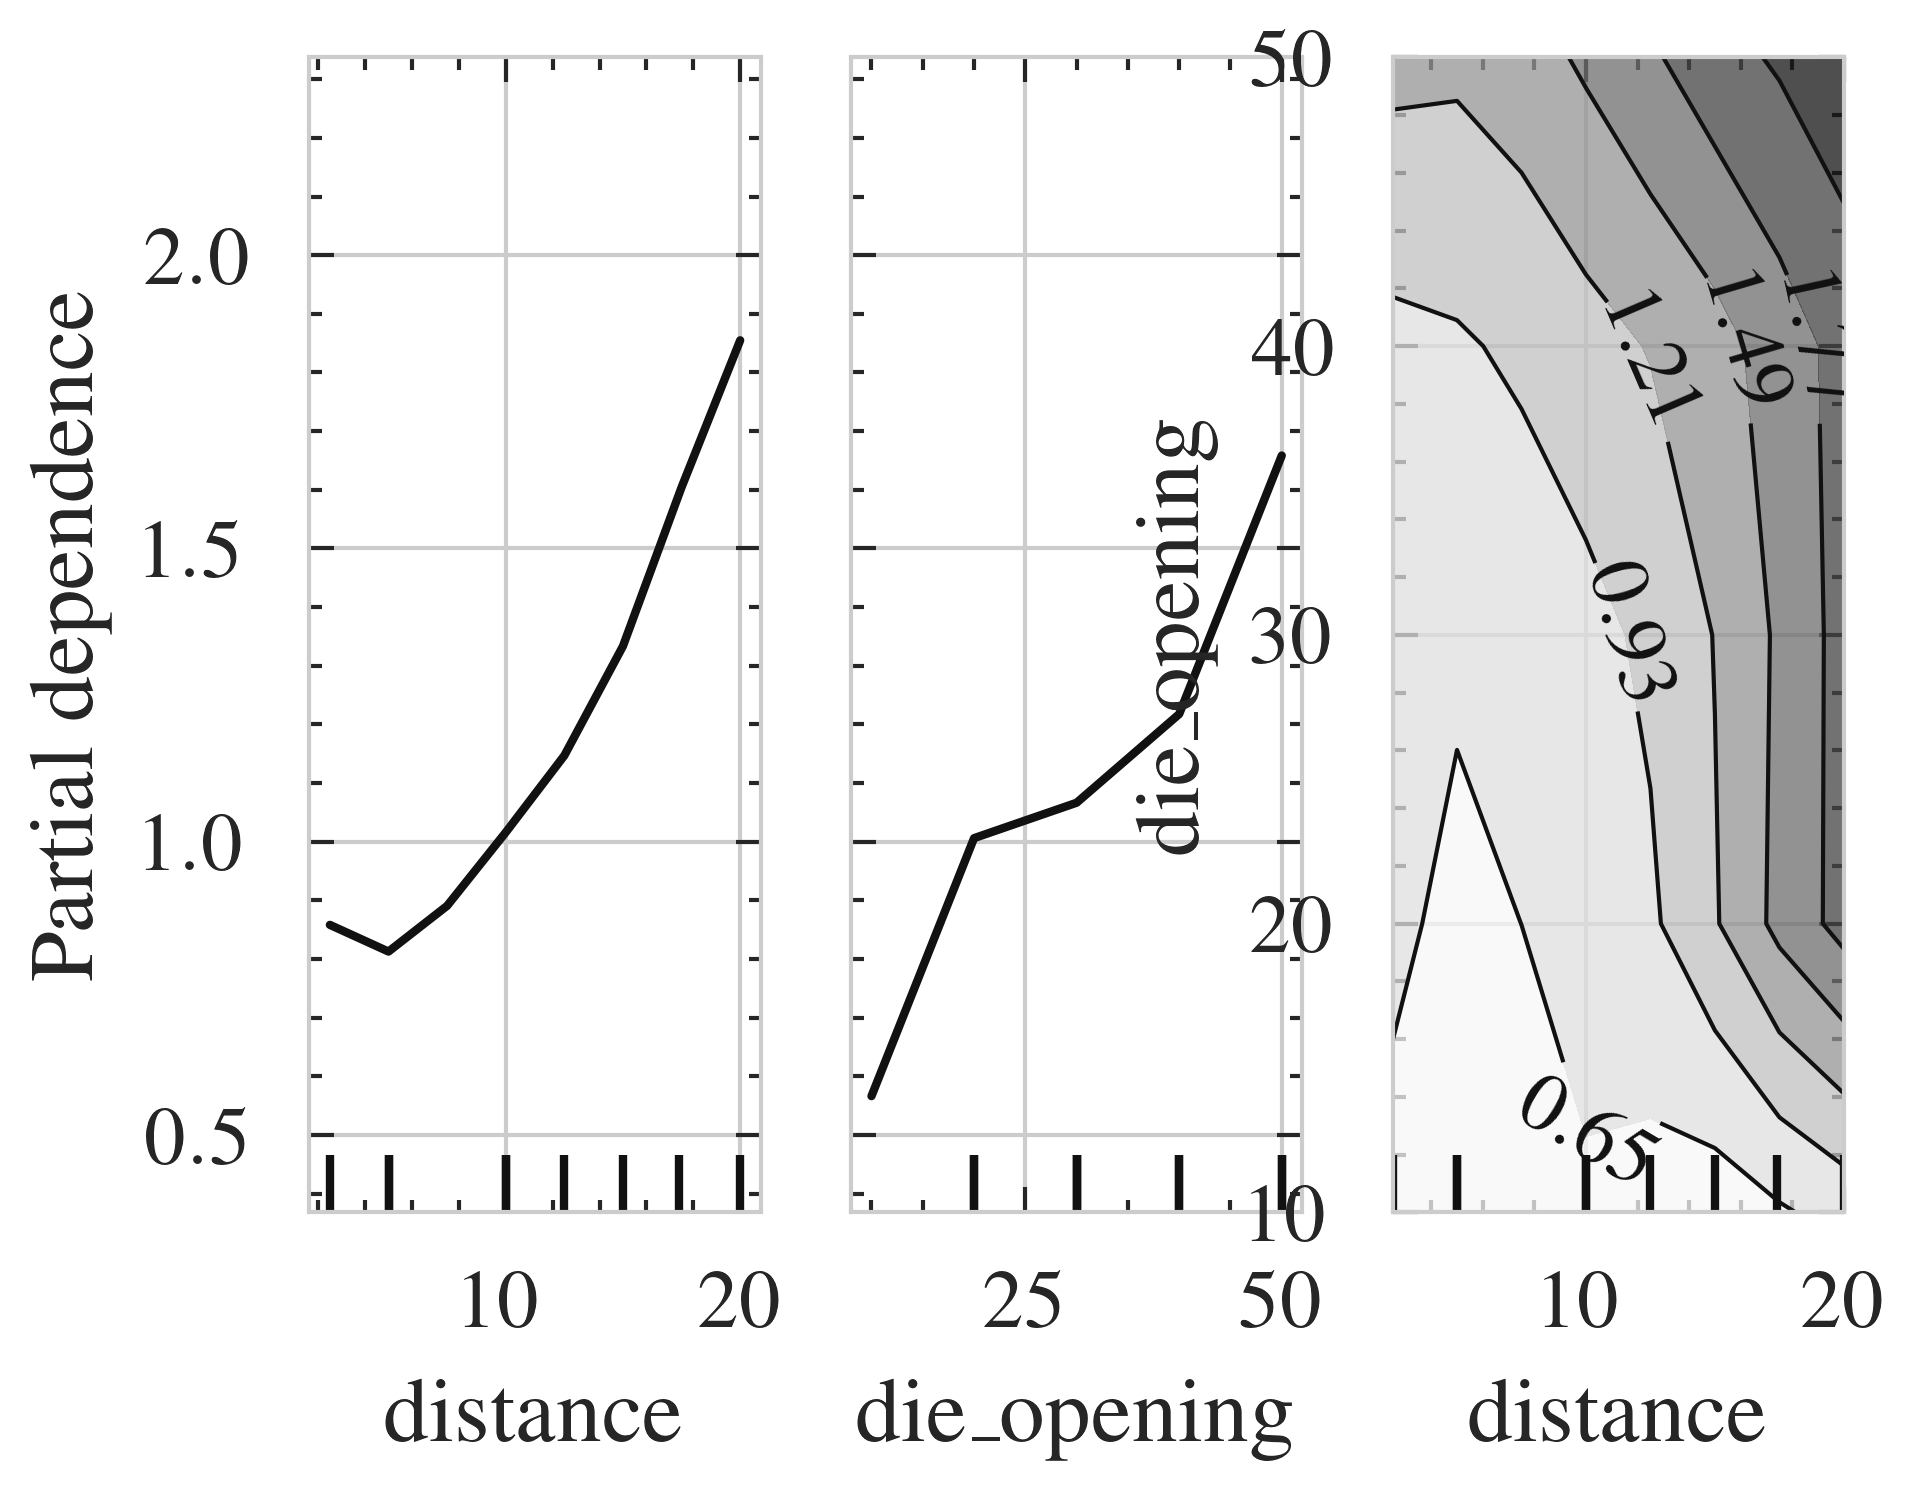
\includegraphics[width=0.9\textwidth]{chap5/images/pdp_distance_die_opening}
    \end{tcolorbox}
    \caption{DPD distance and die opening}
    \label{fig:dpd-distance-die-opening}
\end{figure}

\subsection*{Local Model Agnostic Methods}
Local interpretability refers to the ability to understand the behavior of the model for a
specific instance and is often used to explain the predictions of a model.
Model agnostic methods can be used to explain the predictions of any model type~\cite{
    molnar2020interpretable}.

Local methods rely on interpreting individual instances from a dataset, and as such, it is
crucial to select representative samples.
One way to achieve this is by considering the V/t ratio of each instance.

\subsection{LIME}\label{subsec:lime}
The LIME method stands for Local interpretable model-agnostic explanations
and a model itself that can be used to explain the predictions of any machine
learning model, the model is treated as a black-box~\cite{ribeiro2016model}.
To accomplish this, LIME generates a new dataset with permuted samples along with the predictions
made by the black box model for each sample.
Using this dataset, LIME trains an interpretable model that is given weights based on the
proximity of the sampled instance to the instance of interest.
The interpretable model can be any model that is considered interpretable, such as a Liner
Regression or Decision Trees.

This approach allows LIME to provide explanations for individual predictions by approximating the
behavior of the black box model in a localized and interpretable way~\cite[p. 185]{
    molnar2020interpretable}.

\cite{molnar2020interpretable} express local surrogate models like LIME as follows:

\begin{tcolorbox}[arc=0pt,boxrule=0.5pt]
    \begin{equation}
        explanation(x) = arg\; min\underset{g \in G}\; L(f,g,\pi_x) + \Omega(g)
    \end{equation}
\end{tcolorbox}

The model for explaining a certain instance $x$ is represented by the model $g$ (such as a
linear regression model), which reduces the loss (for example \ac{MSE}), measuring how closely
the explanation aligns with the prediction made by the original model $f$ (for instance, an
\ac{MLP} model).
At the same time, the model complexity $\Omega(g)$ should remain low.
The set of all possible linear regression models is referred to as $G$ , which encompasses all
potential explanations.
The proximity measure, denoted as $\pi_x$ , determines the size of the area surrounding the area
surrounding the instance $x$ that is taken into account for the
explanation~\cite[p. 185]{molnar2020interpretable}.

LIME mainly provides instance explanations in the form of feature importance values.
It can show the predicted values along with the explanations on how which features contributed
in which direction to the prediction.
This can be seen similar to PDP plots but instead of showing the average effect of a feature
on the the overall prediction of the model, it shows the effect of a feature on the prediction
for a specific instance.
One instance in this case consists of the thickness, distance die opening and the corresponding
spring back value.


\textit{If I have questions for specific instances I should put them here.}


\section{Demonstration}\label{sec:demonstration}

\subsection{Comparison of the Models}\label{subsec:overall-comparison-model-performance}
This section will showcase the outcomes generated by the trained models in more detail and
will also discuss the results in relation to the research questions.
This is done in this section to find out the best perfoming models.
These models will be researched in more detail later with the help of model-agnostic
methods to explain the predictions of the models.

In order to evaluate the model's performance without bias, each test case where removed
from the training data set so that the model has not seen the test case before.
This results in a small but notable performance decrease in the test cases, but makes sure that the
results are not biased.

For the interpretation of the next picutres it is relevant to nkow that the target values
repesent the man of all values.
The quality the dataset is but not perfect, and it is possible that there are some outliers in the
dataset.

Figure~\ref{fig:performance-case-a} shows show two chosen test cases for case A with a
V/t-ratio of 20 (\ref{fig:performance-20-1} and 6.6 (\ref{fig:performance-20-3}.

Case~\ref{fig:performance-20-1} with a V/t-ratio of 20 demonstrates the models'
ability to predict the spring with high accuracy.
However, the performance decreases in case b)\ref{fig:performance-20-3} with a V/t-ratio
of 6.6, particularly when predicting the spring backs.
It is likely that there is a measurement error at V = 7.5 in case
b)~\ref{fig:performance-20-3}, causing some models to potentially predict the correct
spring back.

\begin{figure}[H]
    \begin{tcolorbox}[arc=0pt,boxrule=0.5pt]
        \begin{subfigure}{0.5\textwidth}
            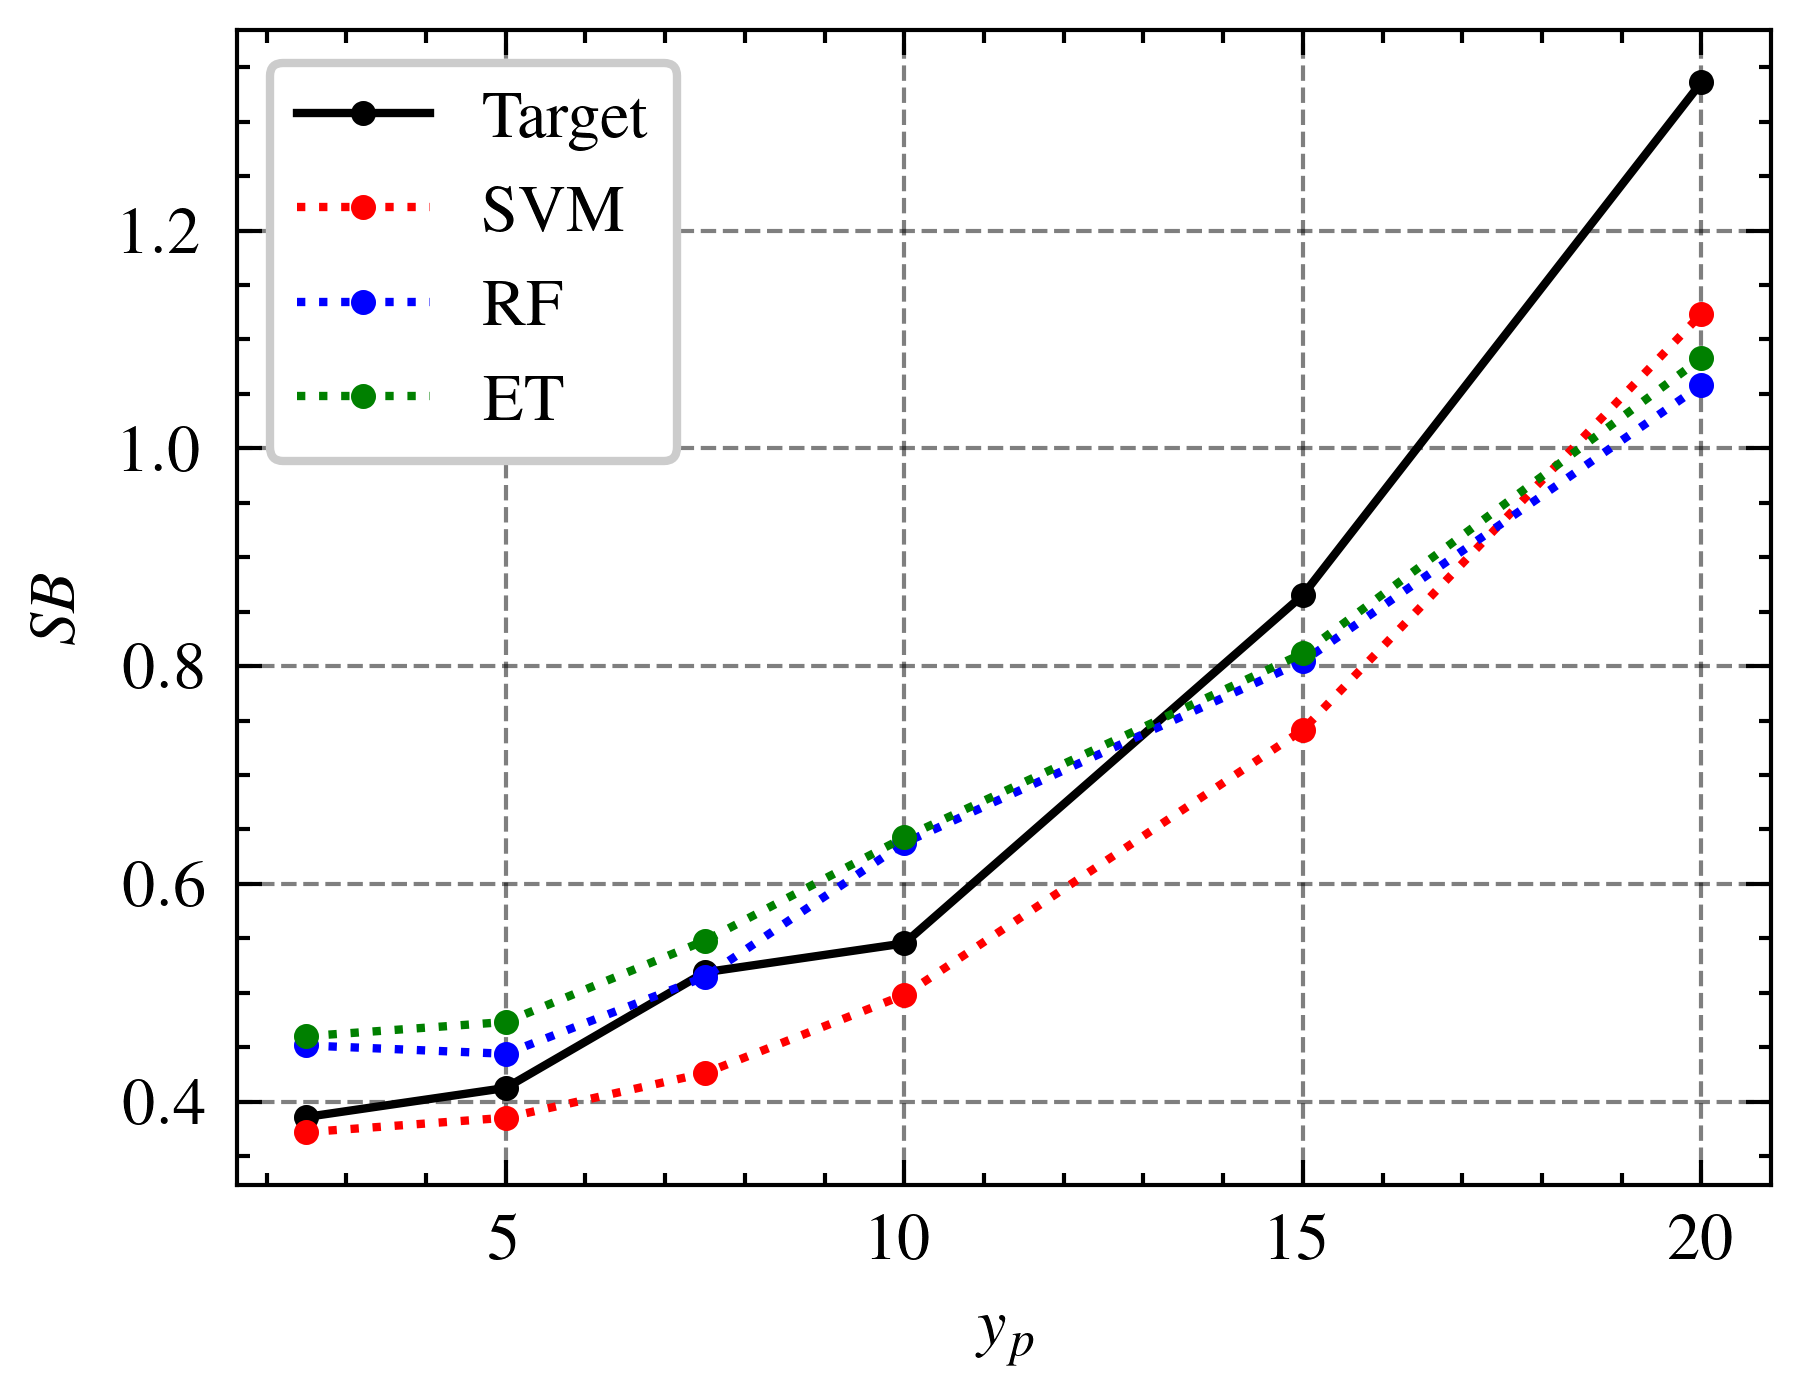
\includegraphics[width=\textwidth]{chap5/images/performance_20_3}
            \caption{V: 20, t: 1}
            \label{fig:performance-20-3-1}
        \end{subfigure}
        \hfill
        \begin{subfigure}{0.5\textwidth}
            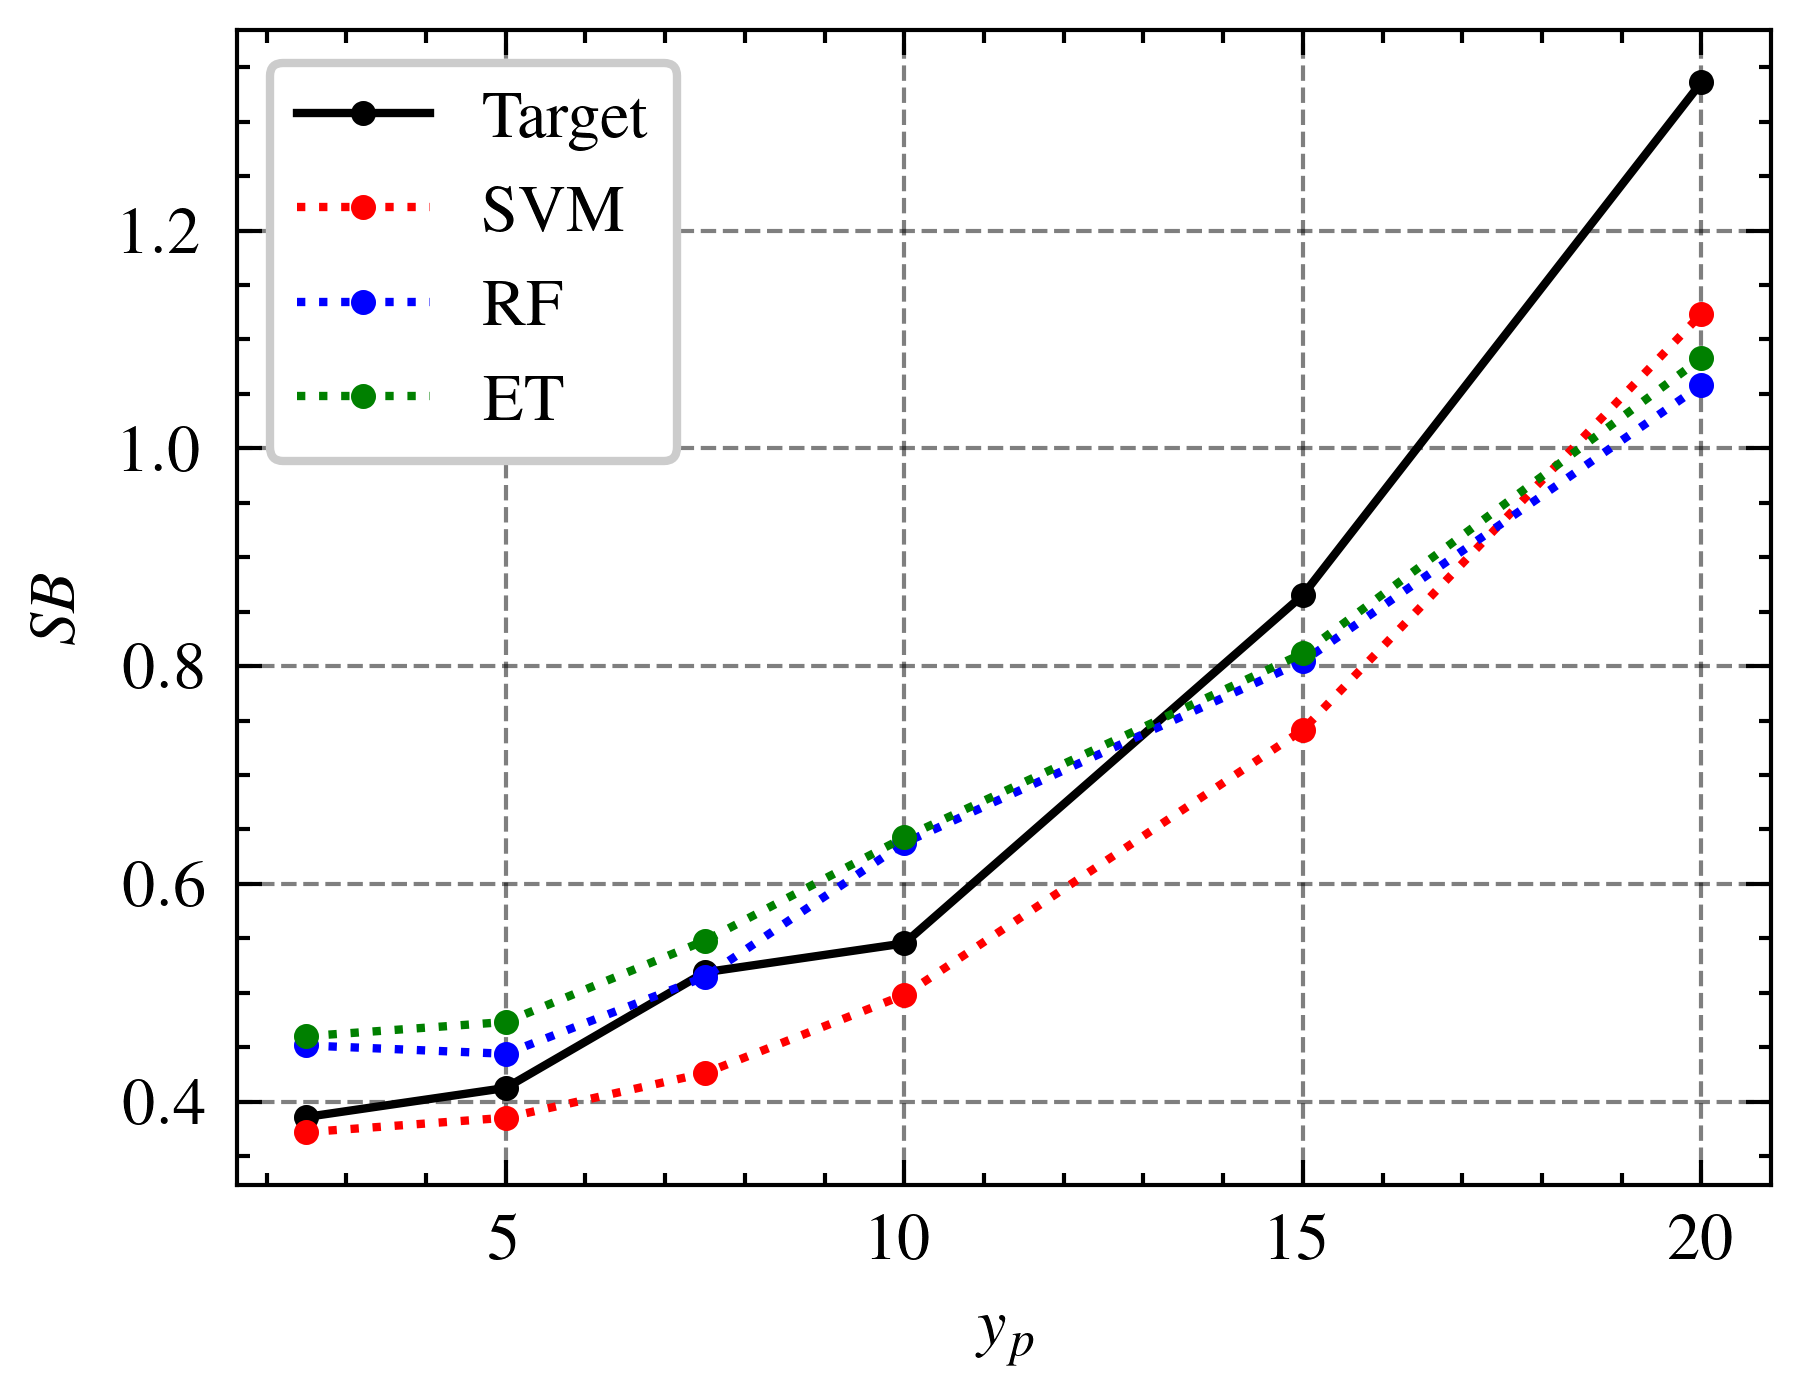
\includegraphics[width=\textwidth]{chap5/images/performance_20_3}
            \caption{V: 20, t: 3}
            \label{fig:performance-20-3-2}
        \end{subfigure}
    \end{tcolorbox}
    \caption{Performance plots for case A}
    \label{fig:performance-case-a}
\end{figure}


Figure~\ref{fig:performance-case-b} displays two selected test series for case B, which indicates
that the V/t ratios fall within the recommended range. These test series produced the best
results compared to cases A and C.

As depicted in figure~\ref{fig:performance-20-1}, both models accurately predicted the spring
back with high precision. The \ac{RF}, \ac{SVM}, and \ac{MLP} models demonstrated similar
performance and produced usable results. Similar findings were observed for figure~\ref{fig
:performance-30_2.0}, where the V/t ratio was different. In this case, the \ac{MLP} model
performed well for \(y_p\) values of 5 and 10, but became inaccurate for higher values. On the
other hand, the \ac{SLP} model consistently produced better results, while the \ac{ET} model
still struggled to perform well.

Overall, it is challenging to identify a clear favorite model based on the performance of the
models in these test series.
While some models performed better than others for specific variables or scenarios, the
differences were not significant enough to identify a clear winner.
Therefore, selecting an appropriate model will be decided by the other two cases A and C.

\begin{figure}[H]
    \begin{tcolorbox}[arc=0pt,boxrule=0.5pt]
        \begin{subfigure}{0.5\textwidth}
            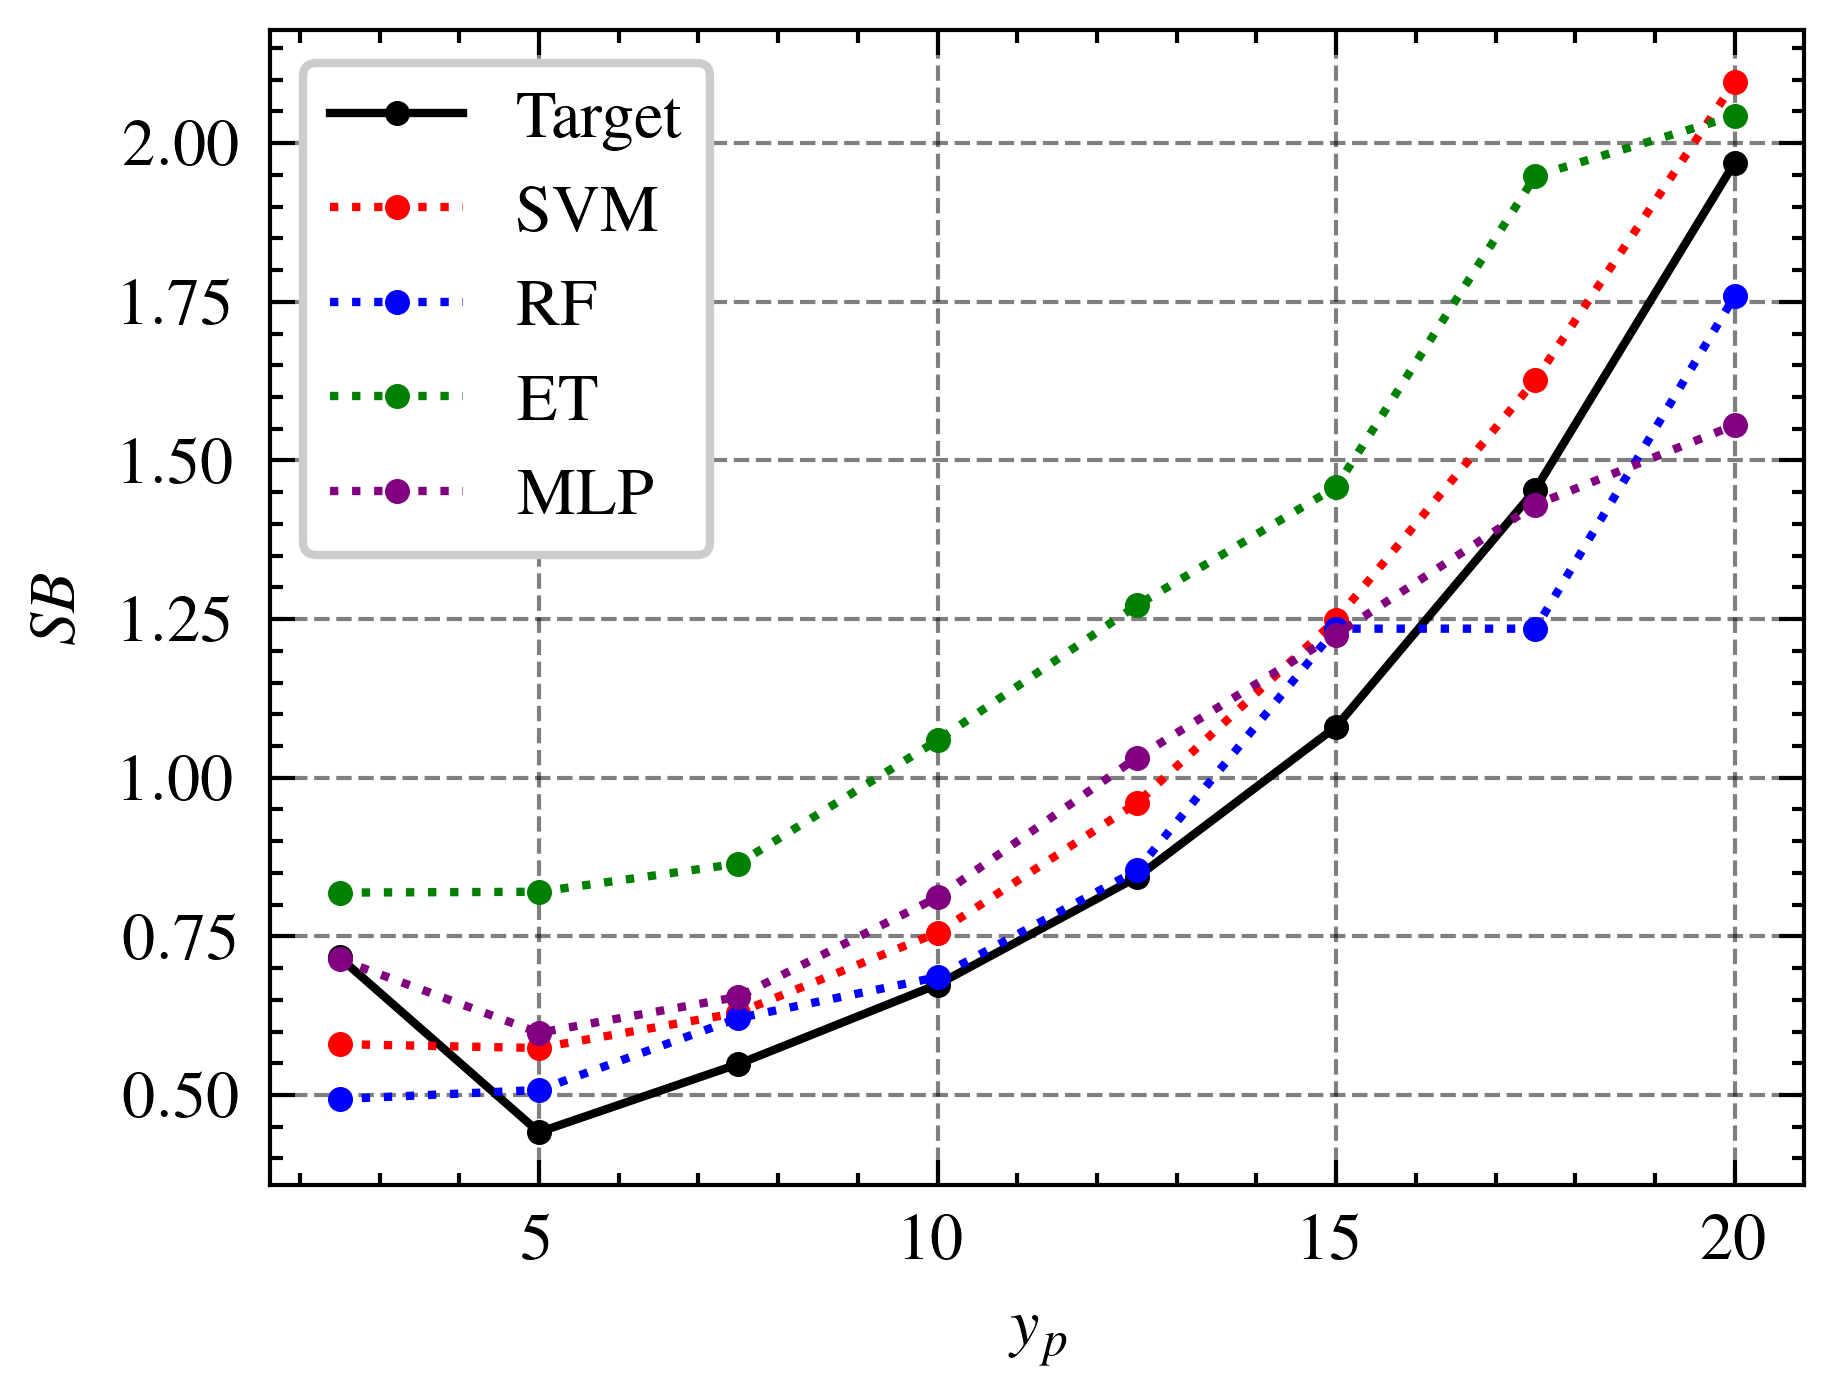
\includegraphics[width=\textwidth]{chap5/images/performance_20_1}
            \caption{V: 20, t: 1}
            \label{fig:performance-20-1}
        \end{subfigure}
        \hfill
        \begin{subfigure}{0.5\textwidth}
            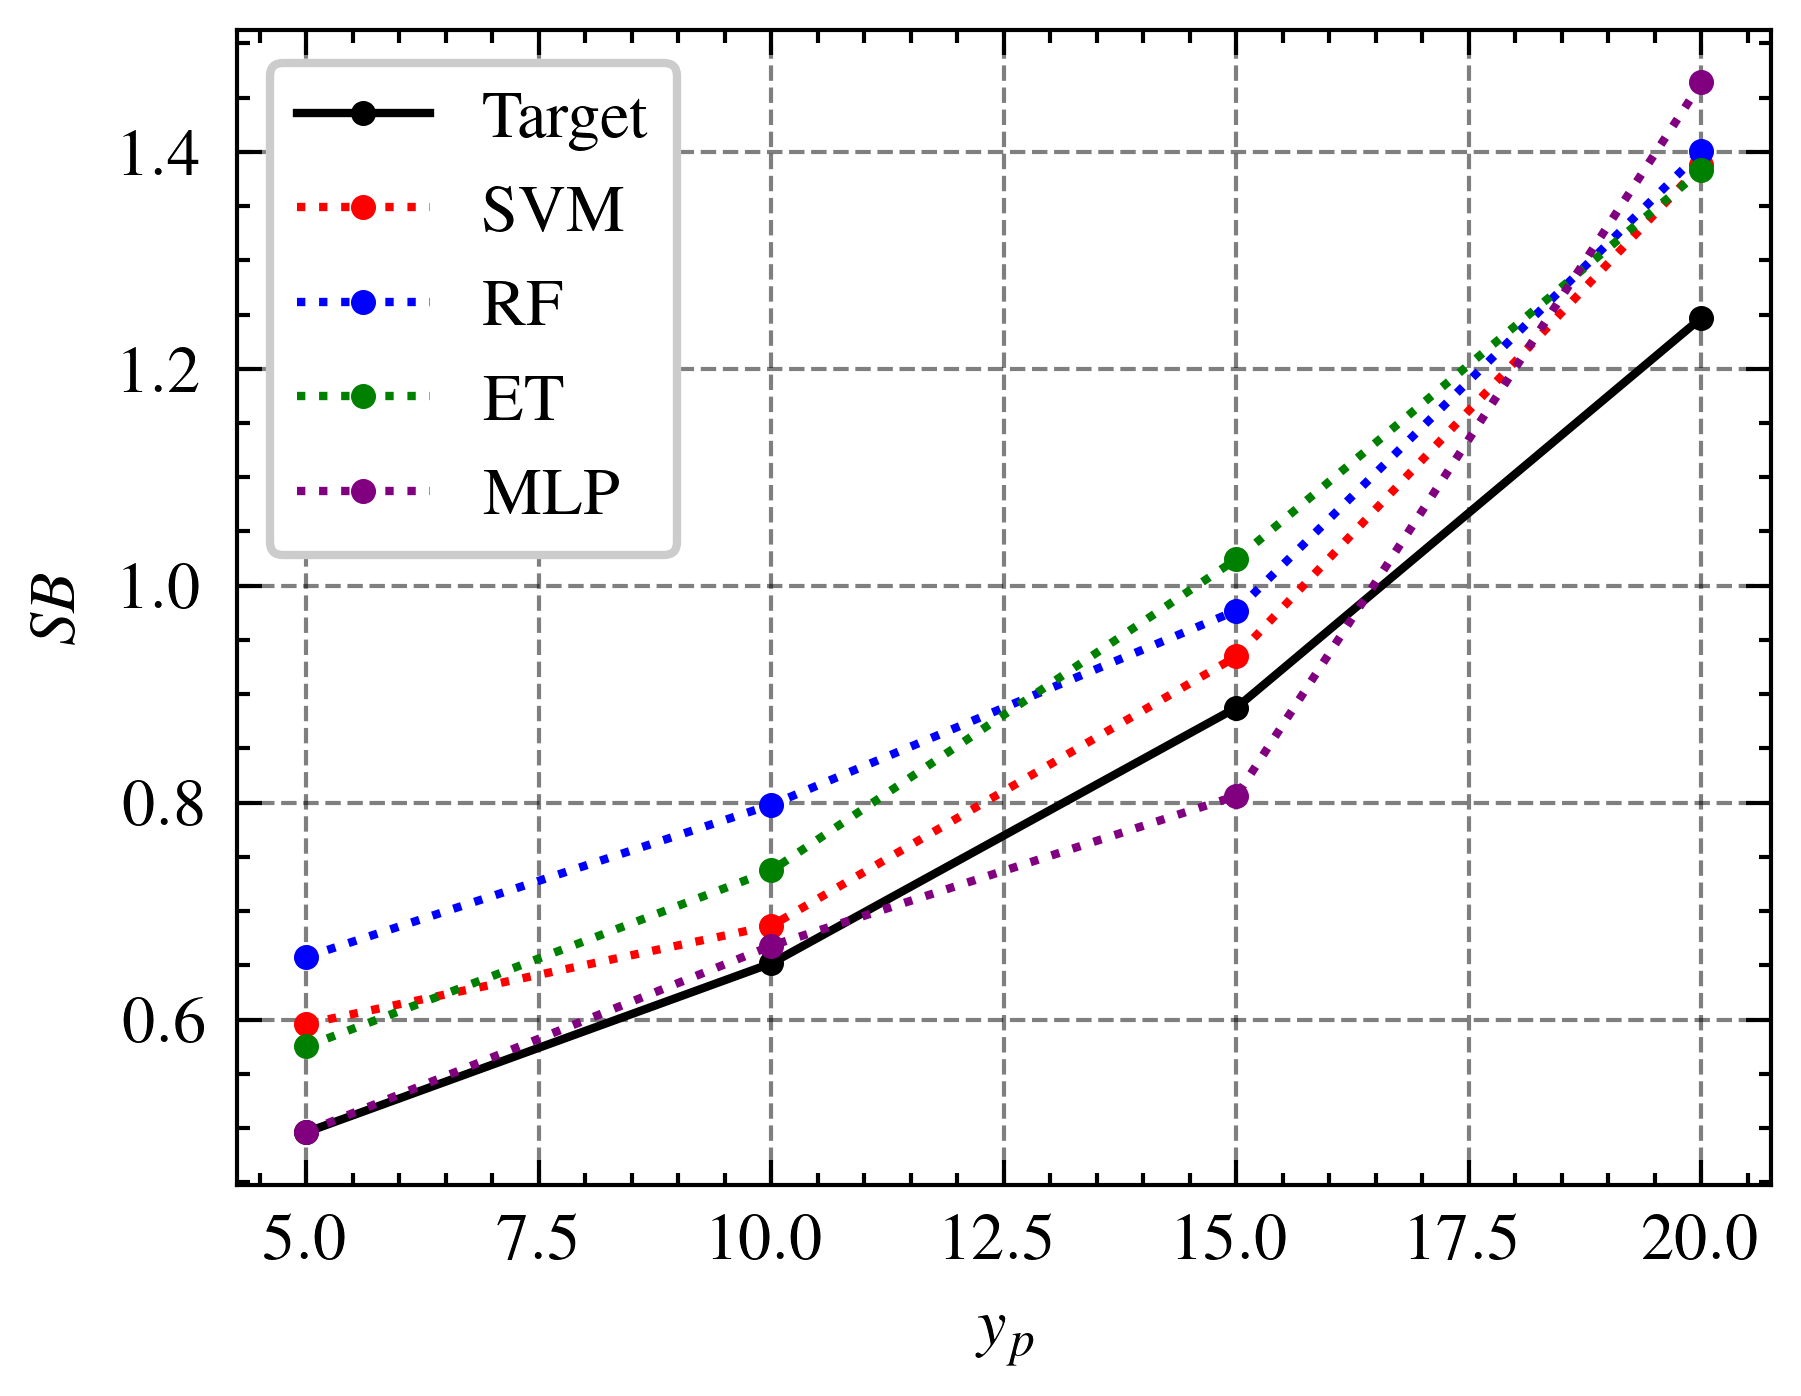
\includegraphics[width=\textwidth]{chap5/images/performance_30_2}
            \caption{V: 30, t: 2}
            \label{fig:performance-30_2.0}
        \end{subfigure}
    \end{tcolorbox}
    \caption{Performance plots for case B}
    \label{fig:performance-case-b}
\end{figure}

Case C is the most challenging case, as the V/t ratios are not within the recommended range.
Figure~\ref{fig:performance-case-c} shows the performance of the models for two test series
with V/t ratios of 50 and 100.

The results shown in figure~\ref{fig:performance-50_0.5} are clear.
The results are unusable, as the models are not able to predict the spring back.
In figure ~\ref{fig:performance-50_1} the results look better, the \ac{RF} and \ac{SVM} model
seem to be the most consistent models?

\begin{figure}[H]
    \begin{tcolorbox}[arc=0pt,boxrule=0.5pt]
        \begin{subfigure}{0.5\textwidth}
            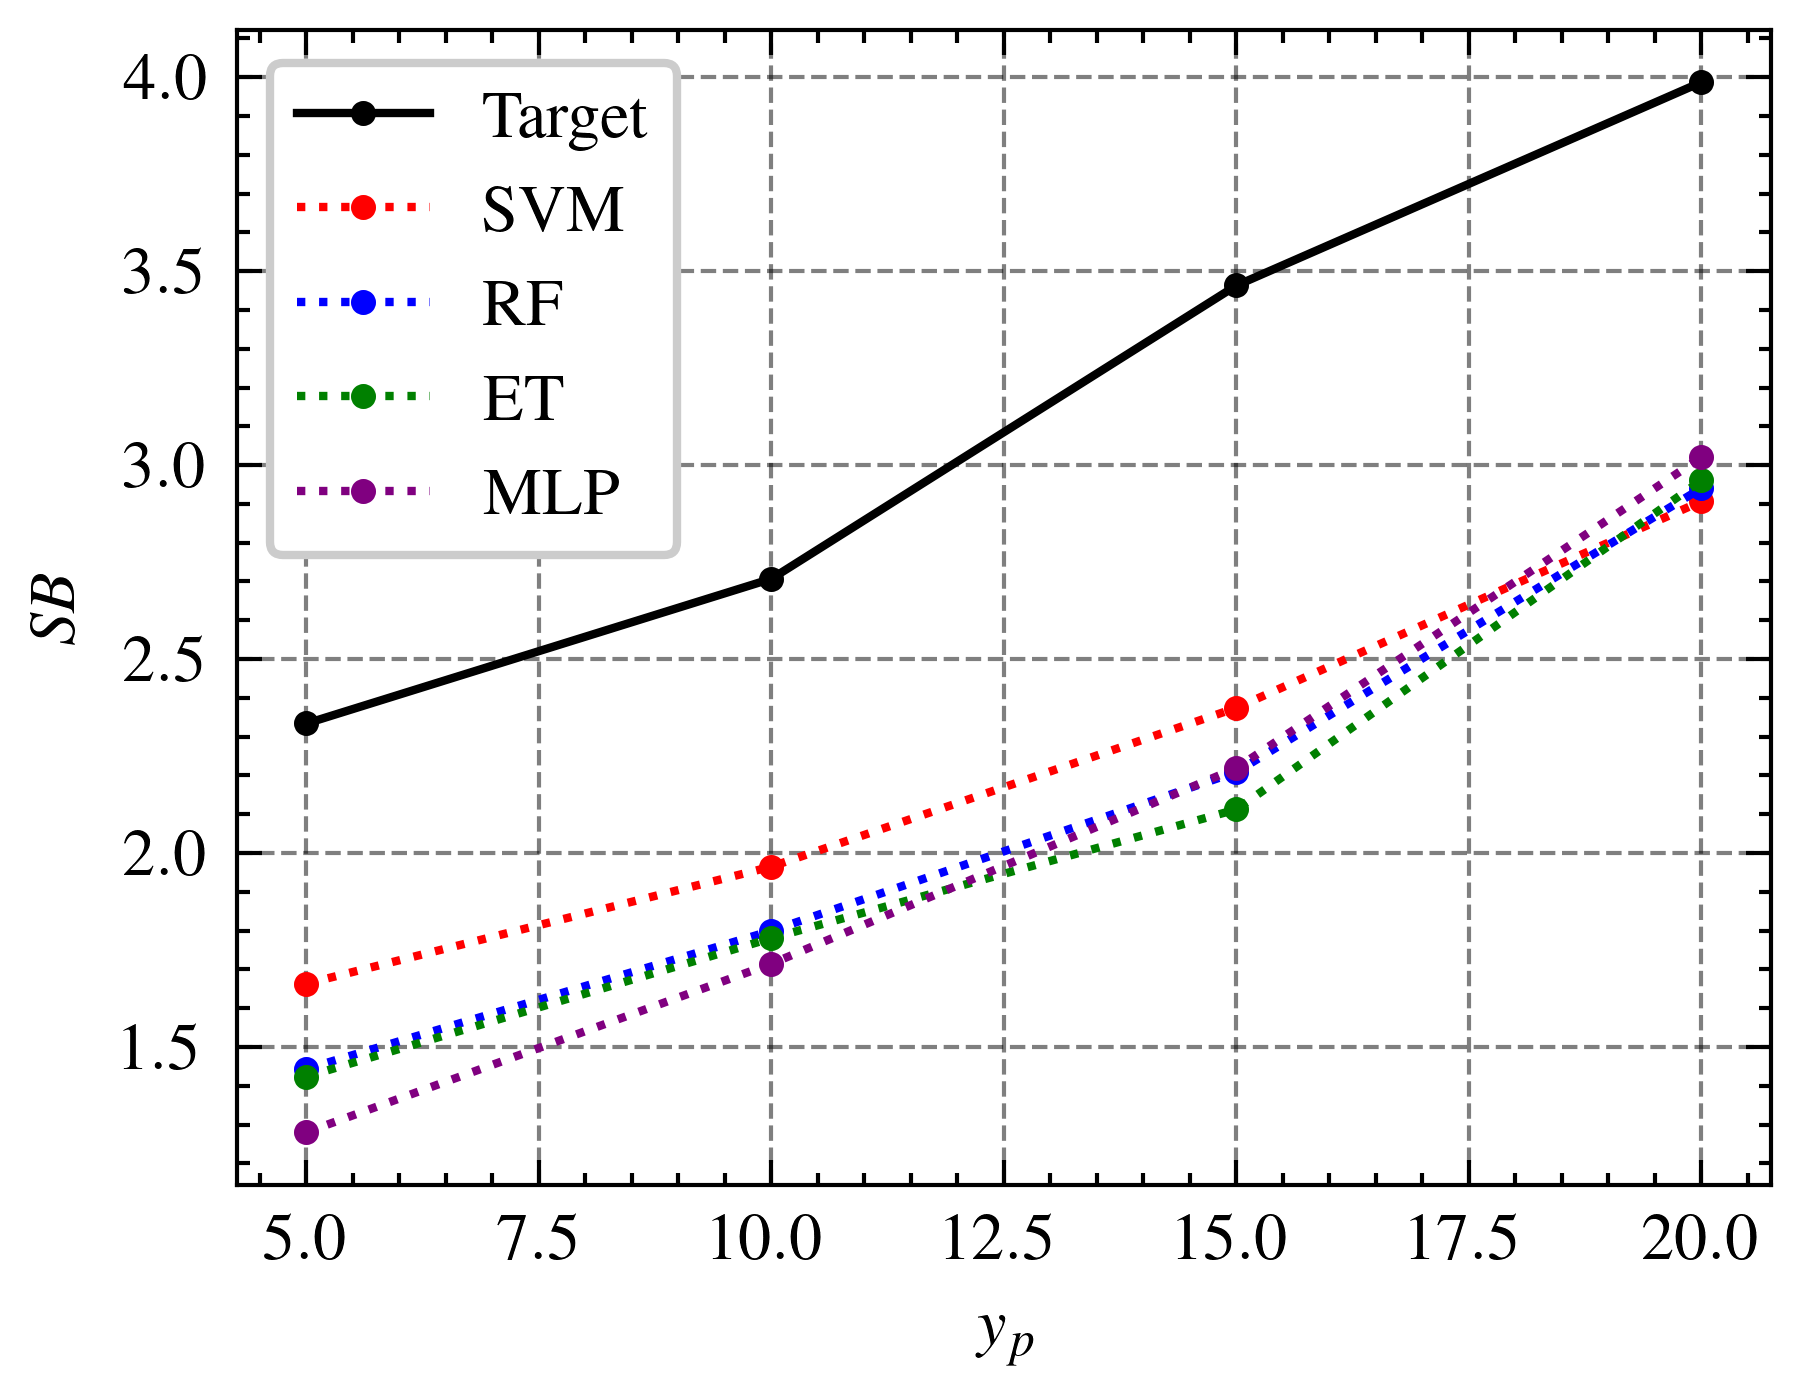
\includegraphics[width=\textwidth]{chap5/images/performance_50_0.5}
            \caption{V: 50, t: 0.5}
            \label{fig:performance-50_0.5}
        \end{subfigure}
        \hfill
        \begin{subfigure}{0.5\textwidth}
            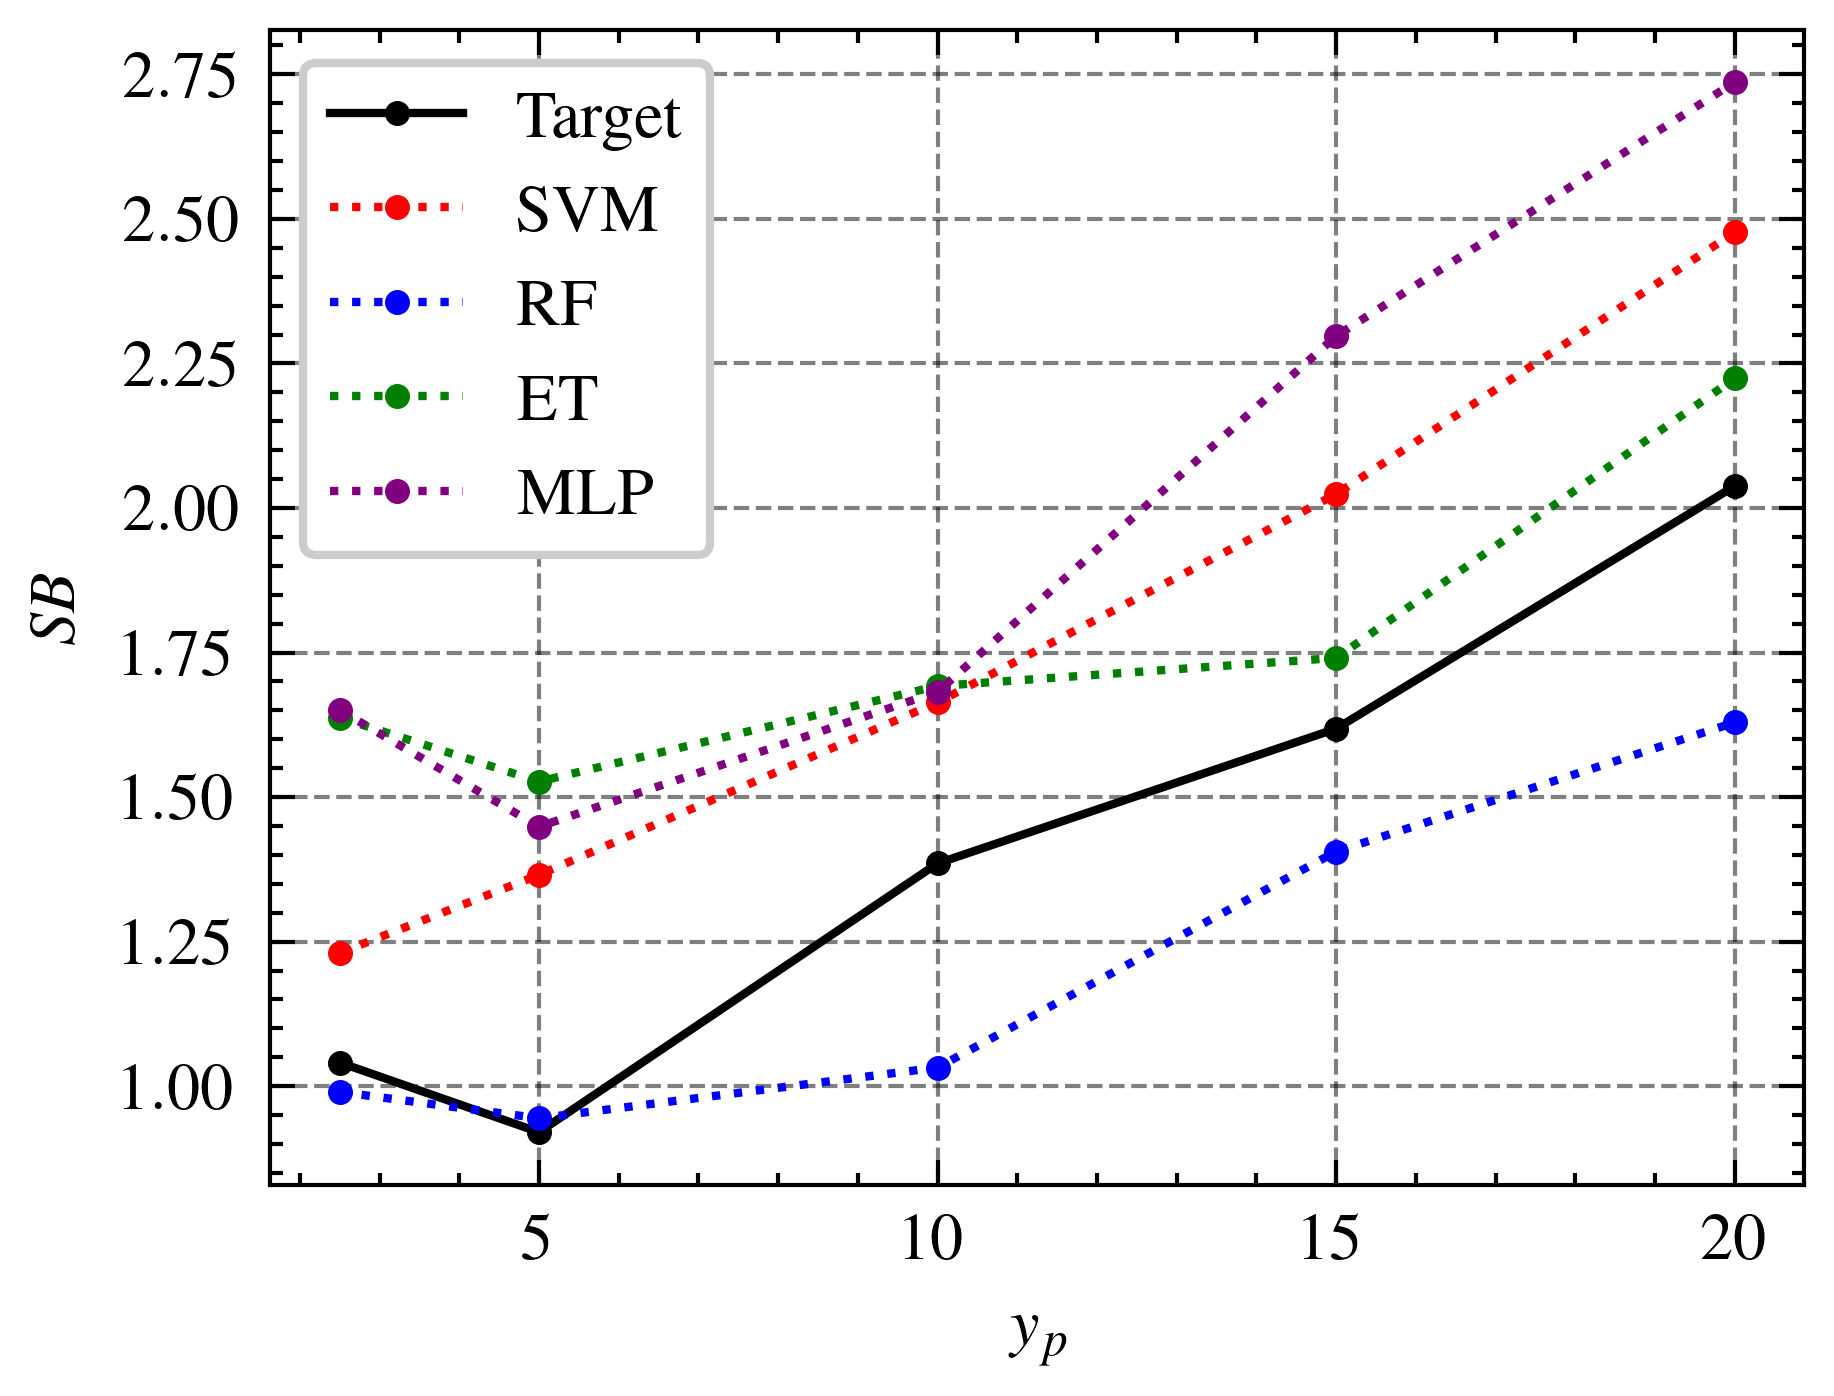
\includegraphics[width=\textwidth]{chap5/images/performance_50_1}
            \caption{V: 50, t: 1}
            \label{fig:performance-50_1}
        \end{subfigure}
    \end{tcolorbox}
    \caption{Performance plots for case C}
    \label{fig:performance-case-c}
\end{figure}

The best overall performing models are the \ac{MLP} and the \ac{SVM} model.
As seen before, the model performs consistent across all thee scenarios, indicating that it can
effectively handle a broad range of V/t ratios also outside the recommended industry guidelines
range.
Therefore the chosen models for more detailed analysis are the \ac{MLP} and the \ac{SVM} model.

Overall it can be said that the models are able to predict the spring back with high accuracy.
For bad predictions the error is less than 0.25 mm, which is within the tolerance of the
most manufacturing processes (This it not true yet).